\chapter{Стабилизация маятника: LQR и фильтр Калмана}
\label{ch:chap6}

\section{Синтез линейно-квадратичного регулятора}
Синтезируем LQR-регулятор на основе линейной модели (\ref{1_model_lin}).

Зададимся матрицами $Q \succ 0$, $R \succ 0$, чем больше значения первой матрицы, тем выше скорость переходного процесса, второй -- меньше сила управления.

\begin{equation}
    Q = \begin{bmatrix}
10 & 0 & 0 & 0\\
0 & 10 & 0 & 0\\
0 & 0 & 10 & 0\\
0 & 0 & 0 & 10
    \end{bmatrix}, \, \, R = 1
\end{equation}

Синтезируем регулятор, минимизирующий функционал качества

\begin{equation}
	J = \int \limits_0^\infty (x^T(t)Qx(t) + u^T(t)Ru(t))dt
\end{equation}
путем решения соответствующего матричного уравнения Риккати при $\nu=1$:

\begin{equation}
	\begin{cases}
		A^TP+PA+Q-\nu PBR^{-1}B^TP = 0,\\
		K = -R^{-1}B^TP
	\end{cases}
\end{equation}

Условия существования решения $P$ выполнено: $Q \succeq 0$, $R \succ 0$, $(A,B)$ -- стабилизируема, $(Q,A)$ -- наблюдаема.

Получим следующее значение матрицы $K$

\begin{equation}
	K = \begin{bmatrix}
		3.2 &   44.3 &  -5720.8   &-2369.3
	\end{bmatrix}
\end{equation}
применим данный регулятор для управления нелинейной системой (\ref{1_model_full}), задавшись начальными условиями $x(0) = [0.01, \, 0.01, \, 0.01, \, 0.01]$, рисунок \ref{6_lqr_1}. Как видим, ситема стабилизируется, причем компоненты вектора $x(t)$ сходятся к нулю за разное время.

\begin{figure}[!h]
	\center{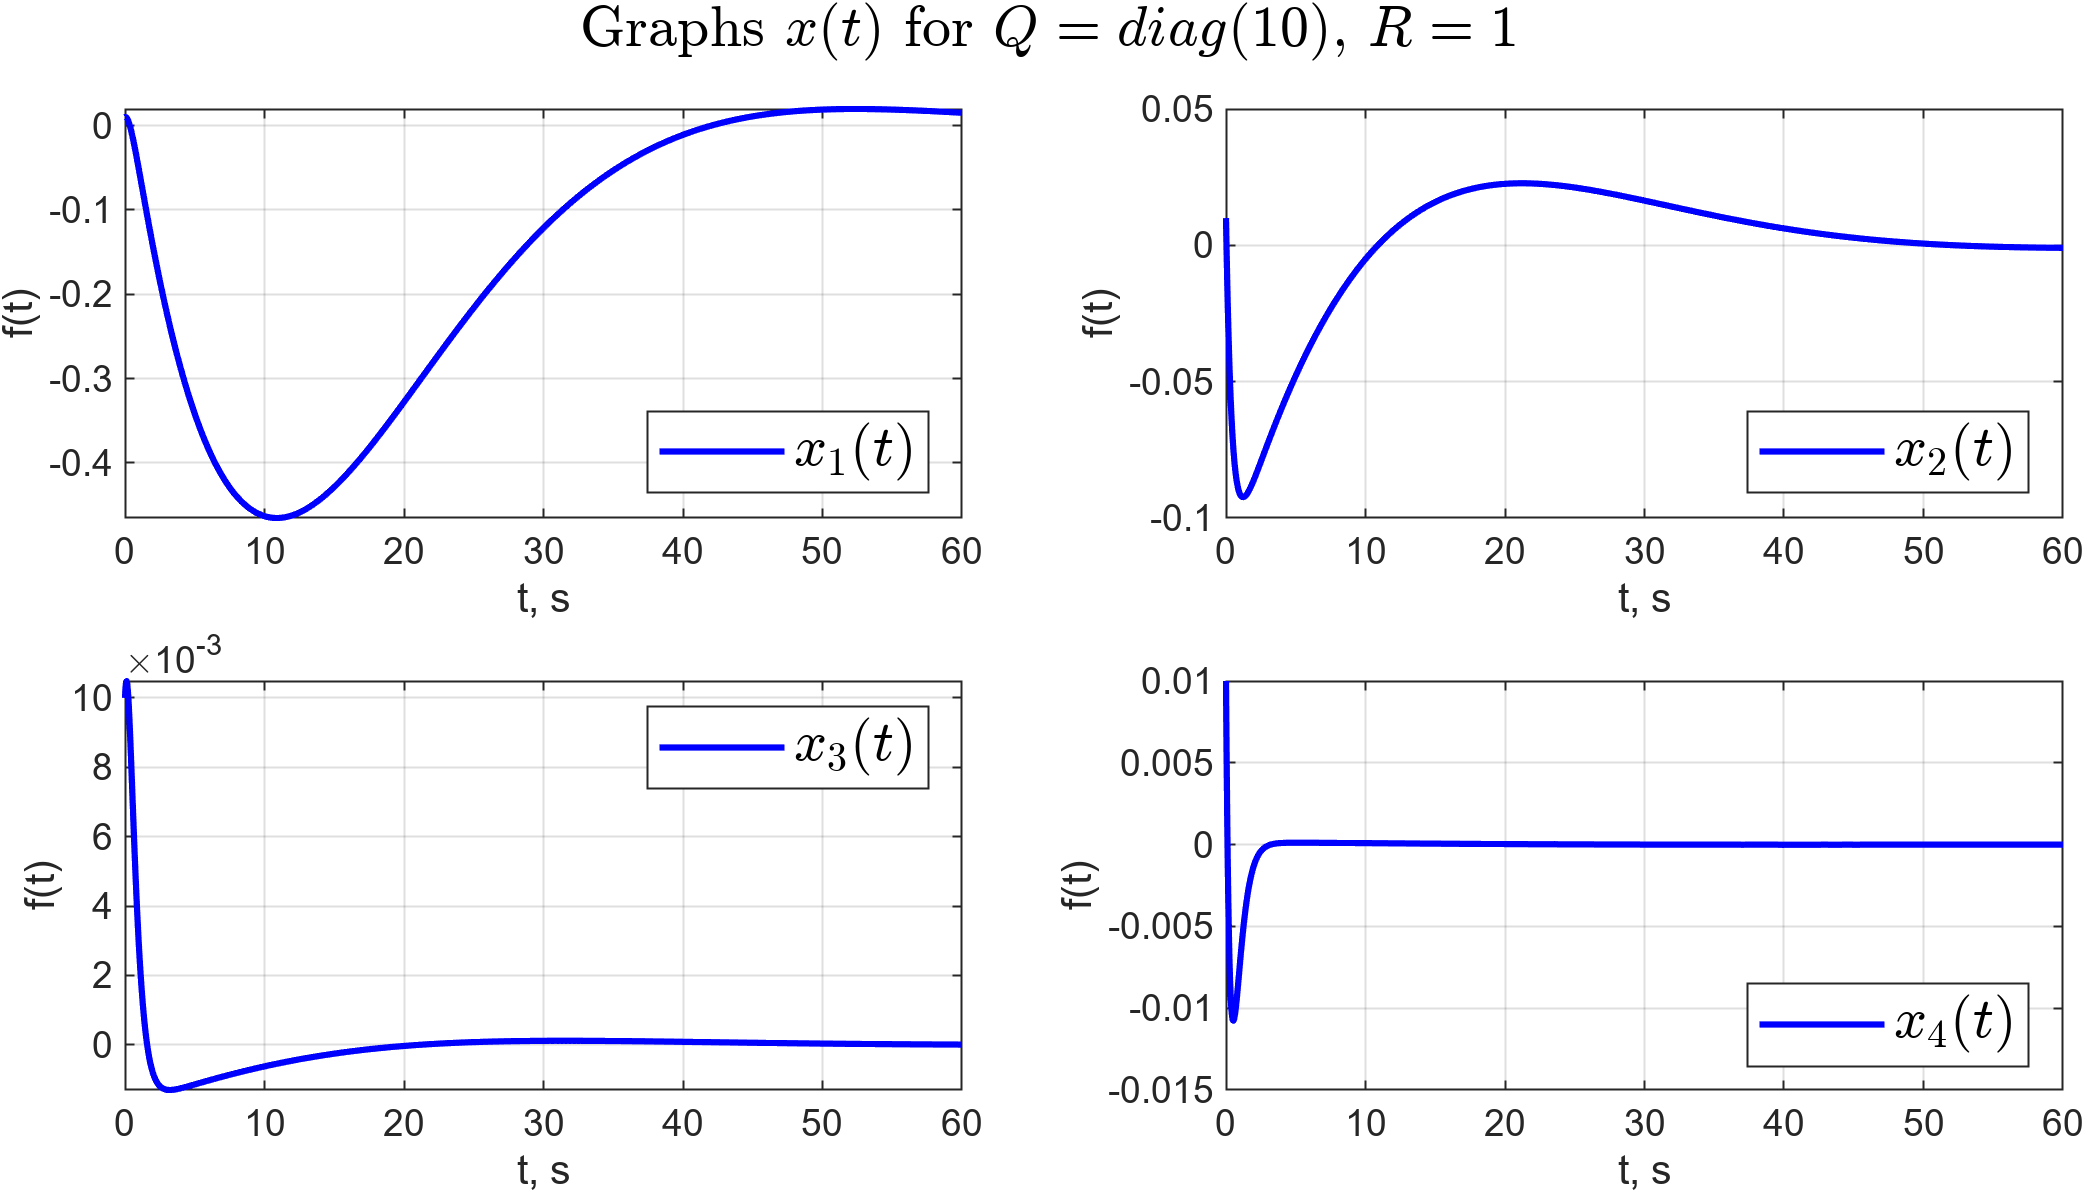
\includegraphics[width=1\linewidth]{pic2/6_lqr_1.png}}
	\caption{Графики $x(t)$ для нелинейной системы.}
	\label{6_lqr_1}
\end{figure}

Исследуем работоспособность синтезированного регулятора при управлении нелинейной системой в зависимости от начальных условий.
\begin{equation*}
	\begin{matrix}
		x(0) = \begin{bmatrix}
			0.01 & 3 & 0.01 & 0.01
		\end{bmatrix}, & x(0) = \begin{bmatrix}
			0.01 & 0.01 & 0.01 & 1.5
		\end{bmatrix},\\
		x(0) = \begin{bmatrix}
			0.01 & 0.01 & \pi /6 & 0.01
		\end{bmatrix}, & x(0) = \begin{bmatrix}
			5 & 0.01 & 0.01 & 0.1
		\end{bmatrix},\\ 
	\end{matrix}
\end{equation*}


\begin{figure}[!h]
	\center{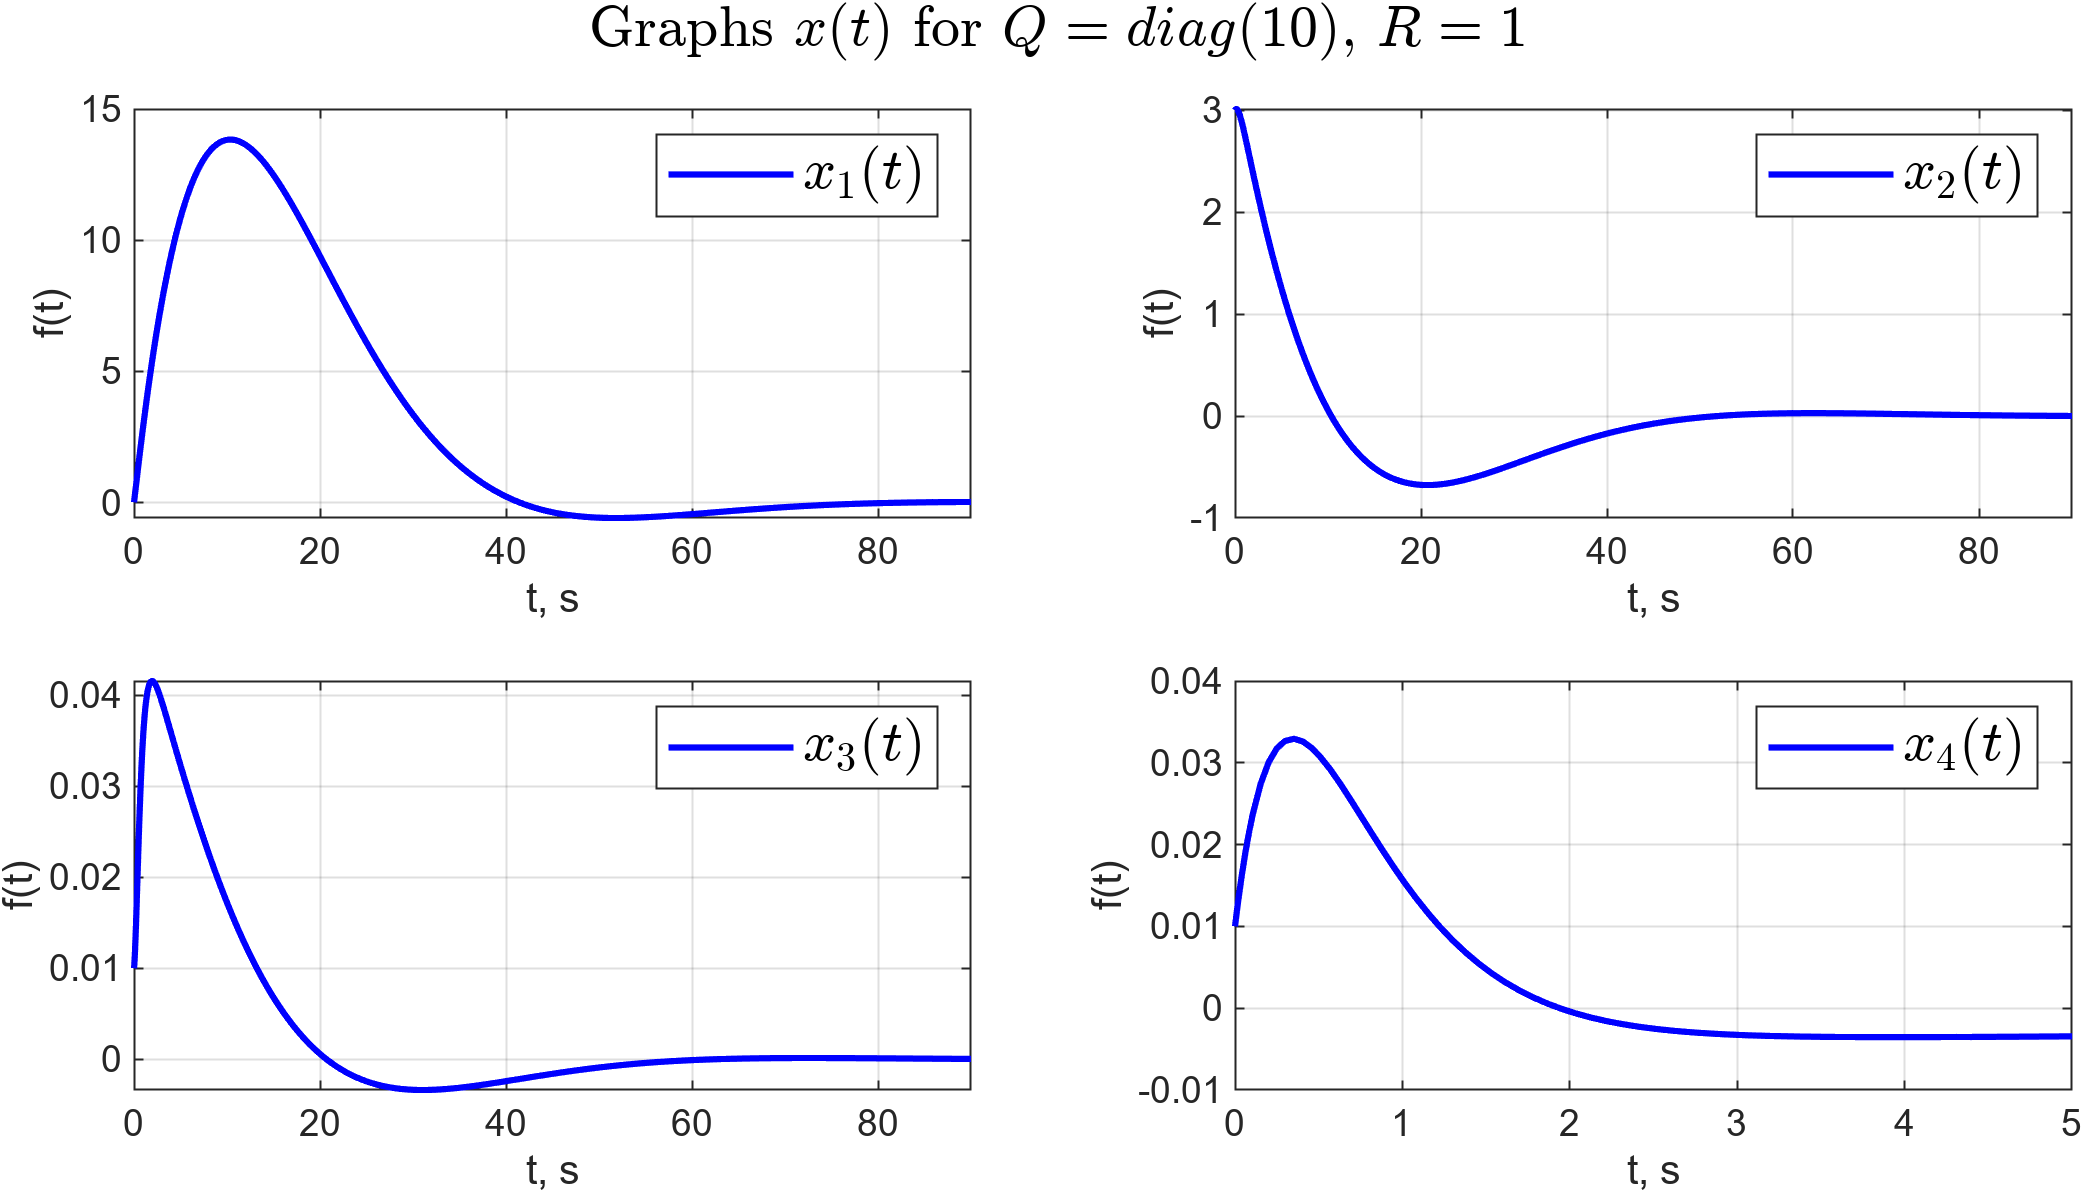
\includegraphics[width=1\linewidth]{pic2/6_lqr_n1.png}}
	\caption{Графики $x(t)$ для нелинейной системы при $x(0)=[0.01, \, \, 3, \, \, 0.01, \, \, 0.01]$.}
	\label{6_lqr_n1}
\end{figure}


\begin{figure}[!h]
	\center{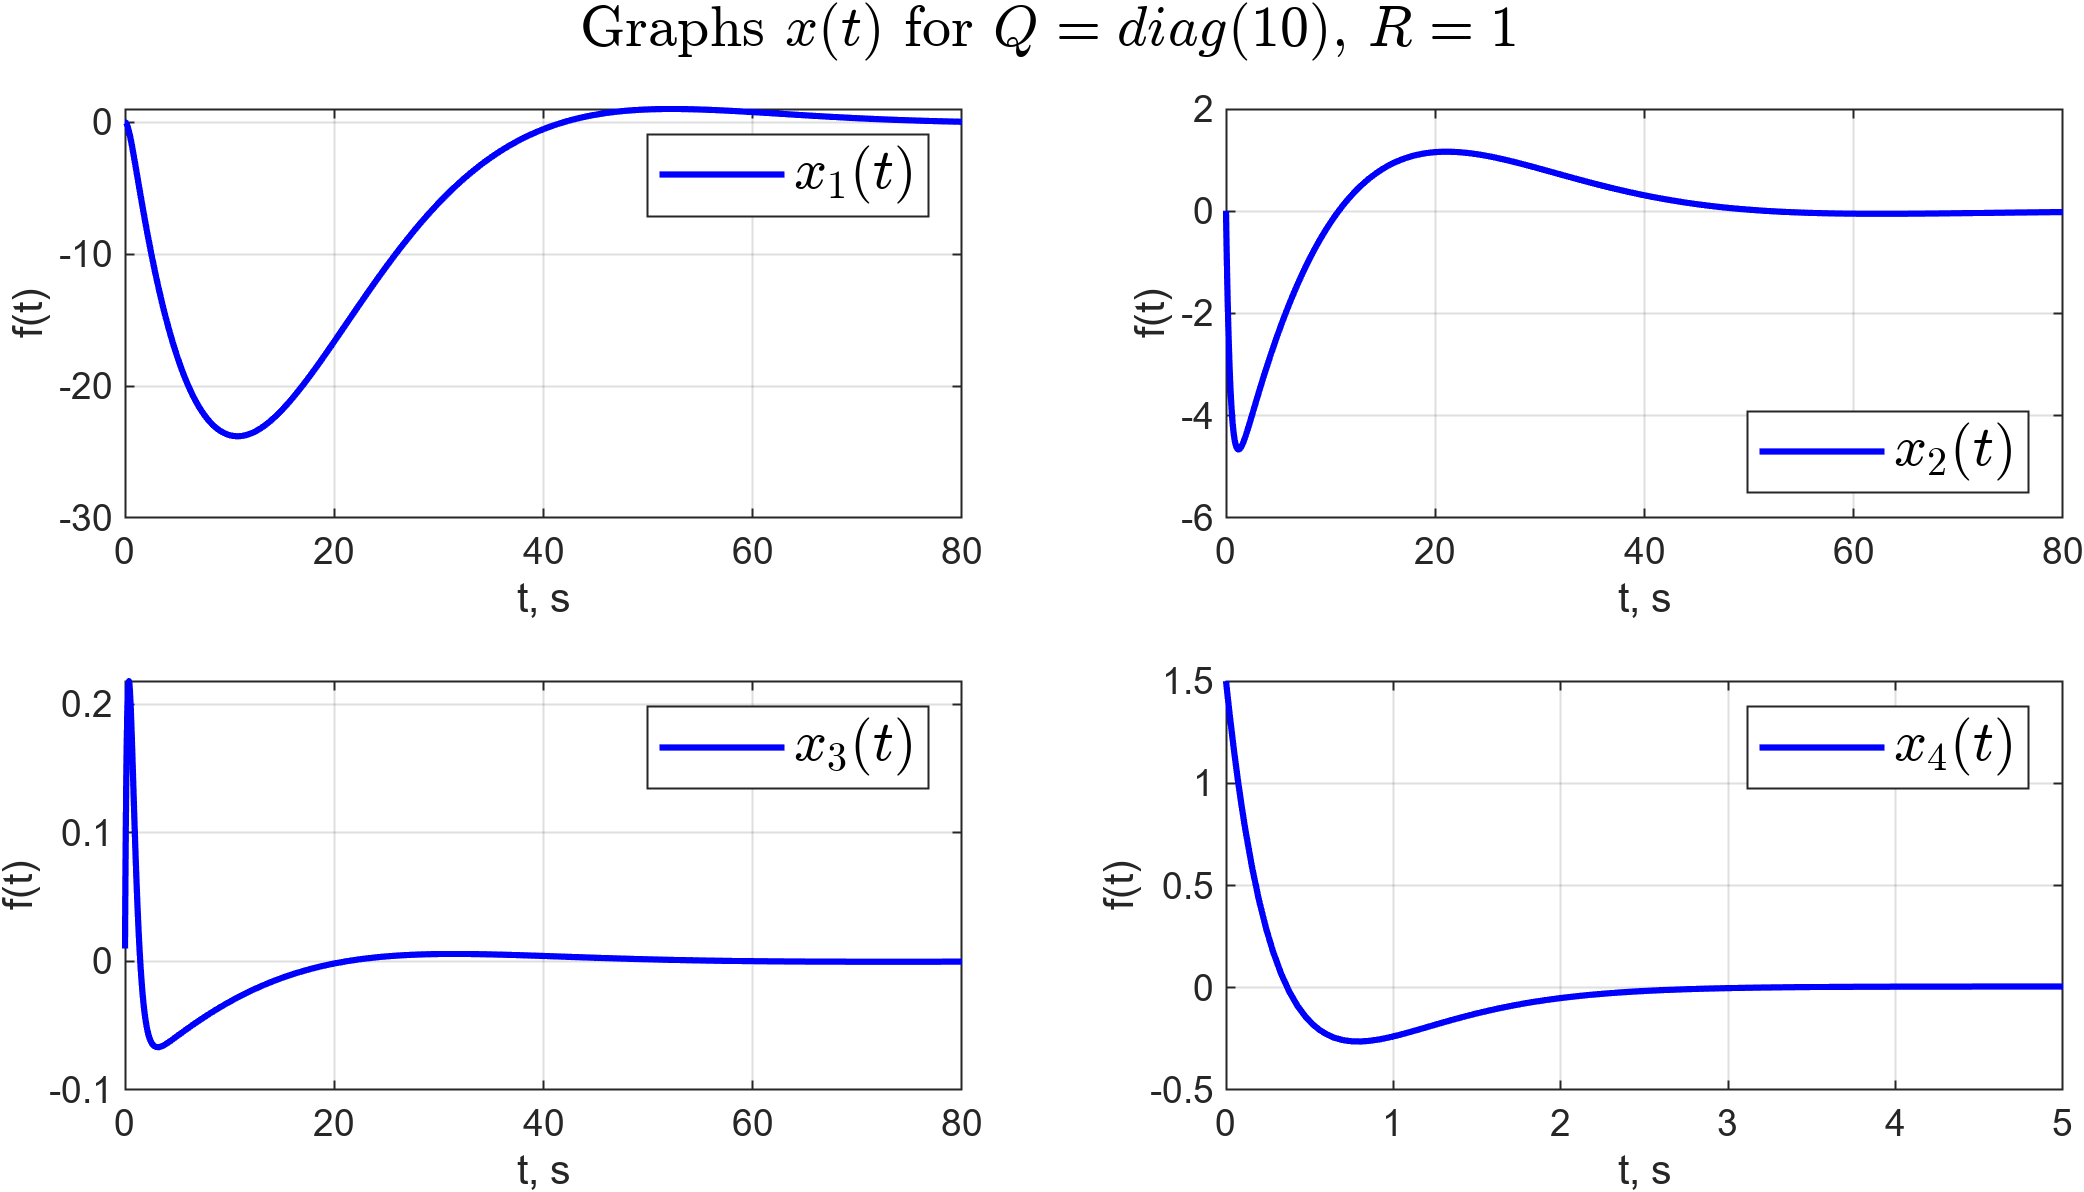
\includegraphics[width=1\linewidth]{pic2/6_lqr_n2.png}}
	\caption{Графики $x(t)$ для нелинейной системы при $x(0)=[0.01, \, \, 0.01, \, \, 0.01, \, \, 1.5]$.}
	\label{6_lqr_n2}
\end{figure}

\begin{figure}[!h]
	\center{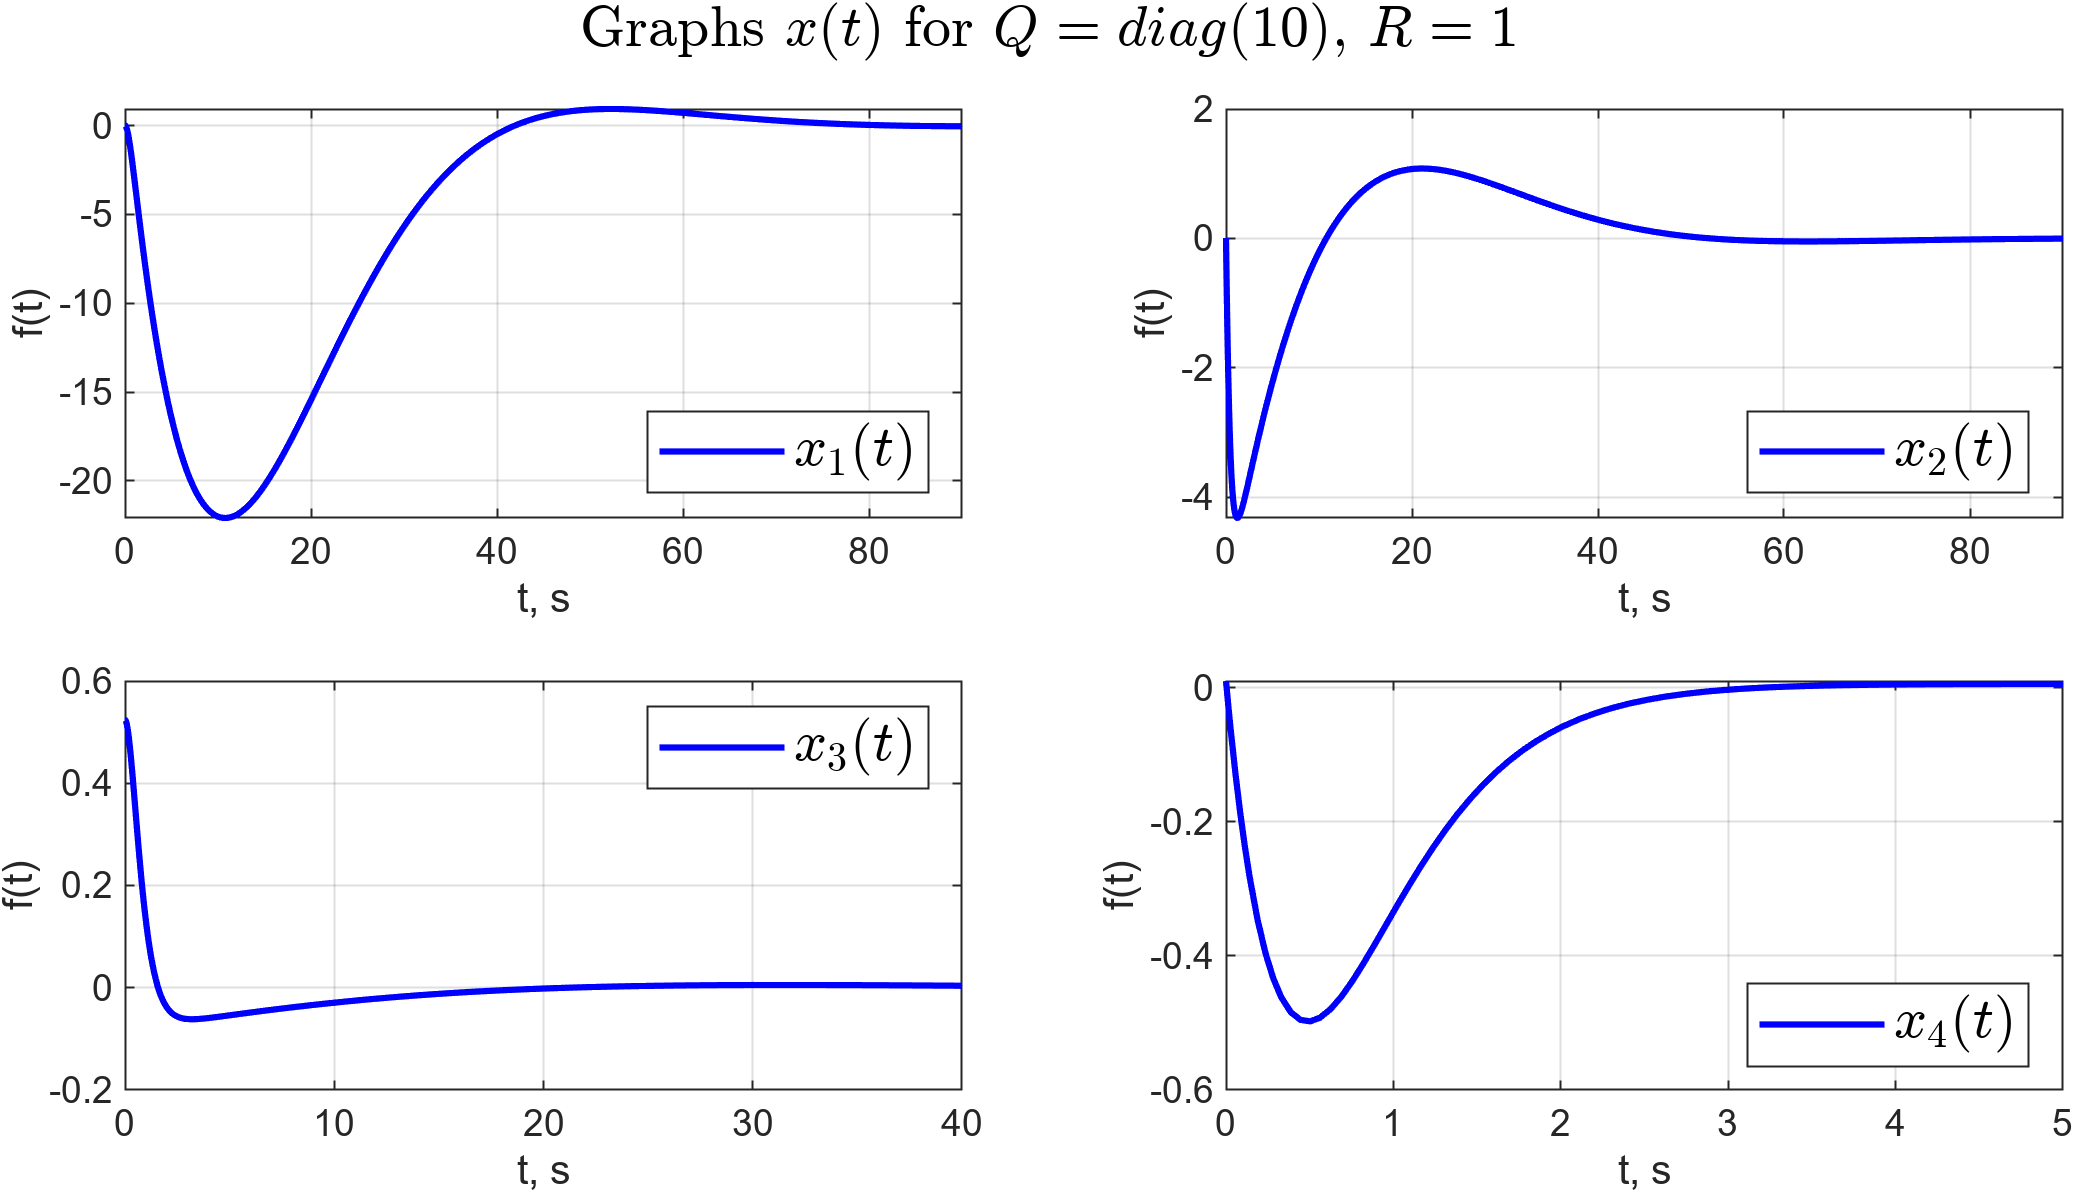
\includegraphics[width=1\linewidth]{pic2/6_lqr_n3.png}}
	\caption{Графики $x(t)$ для нелинейной системы при $x(0)=[0.01, \, \, 0.01, \, \, \pi / 6, \, \, 1.5]$.}
	\label{6_lqr_n3}
\end{figure}

\begin{figure}[!h]
	\center{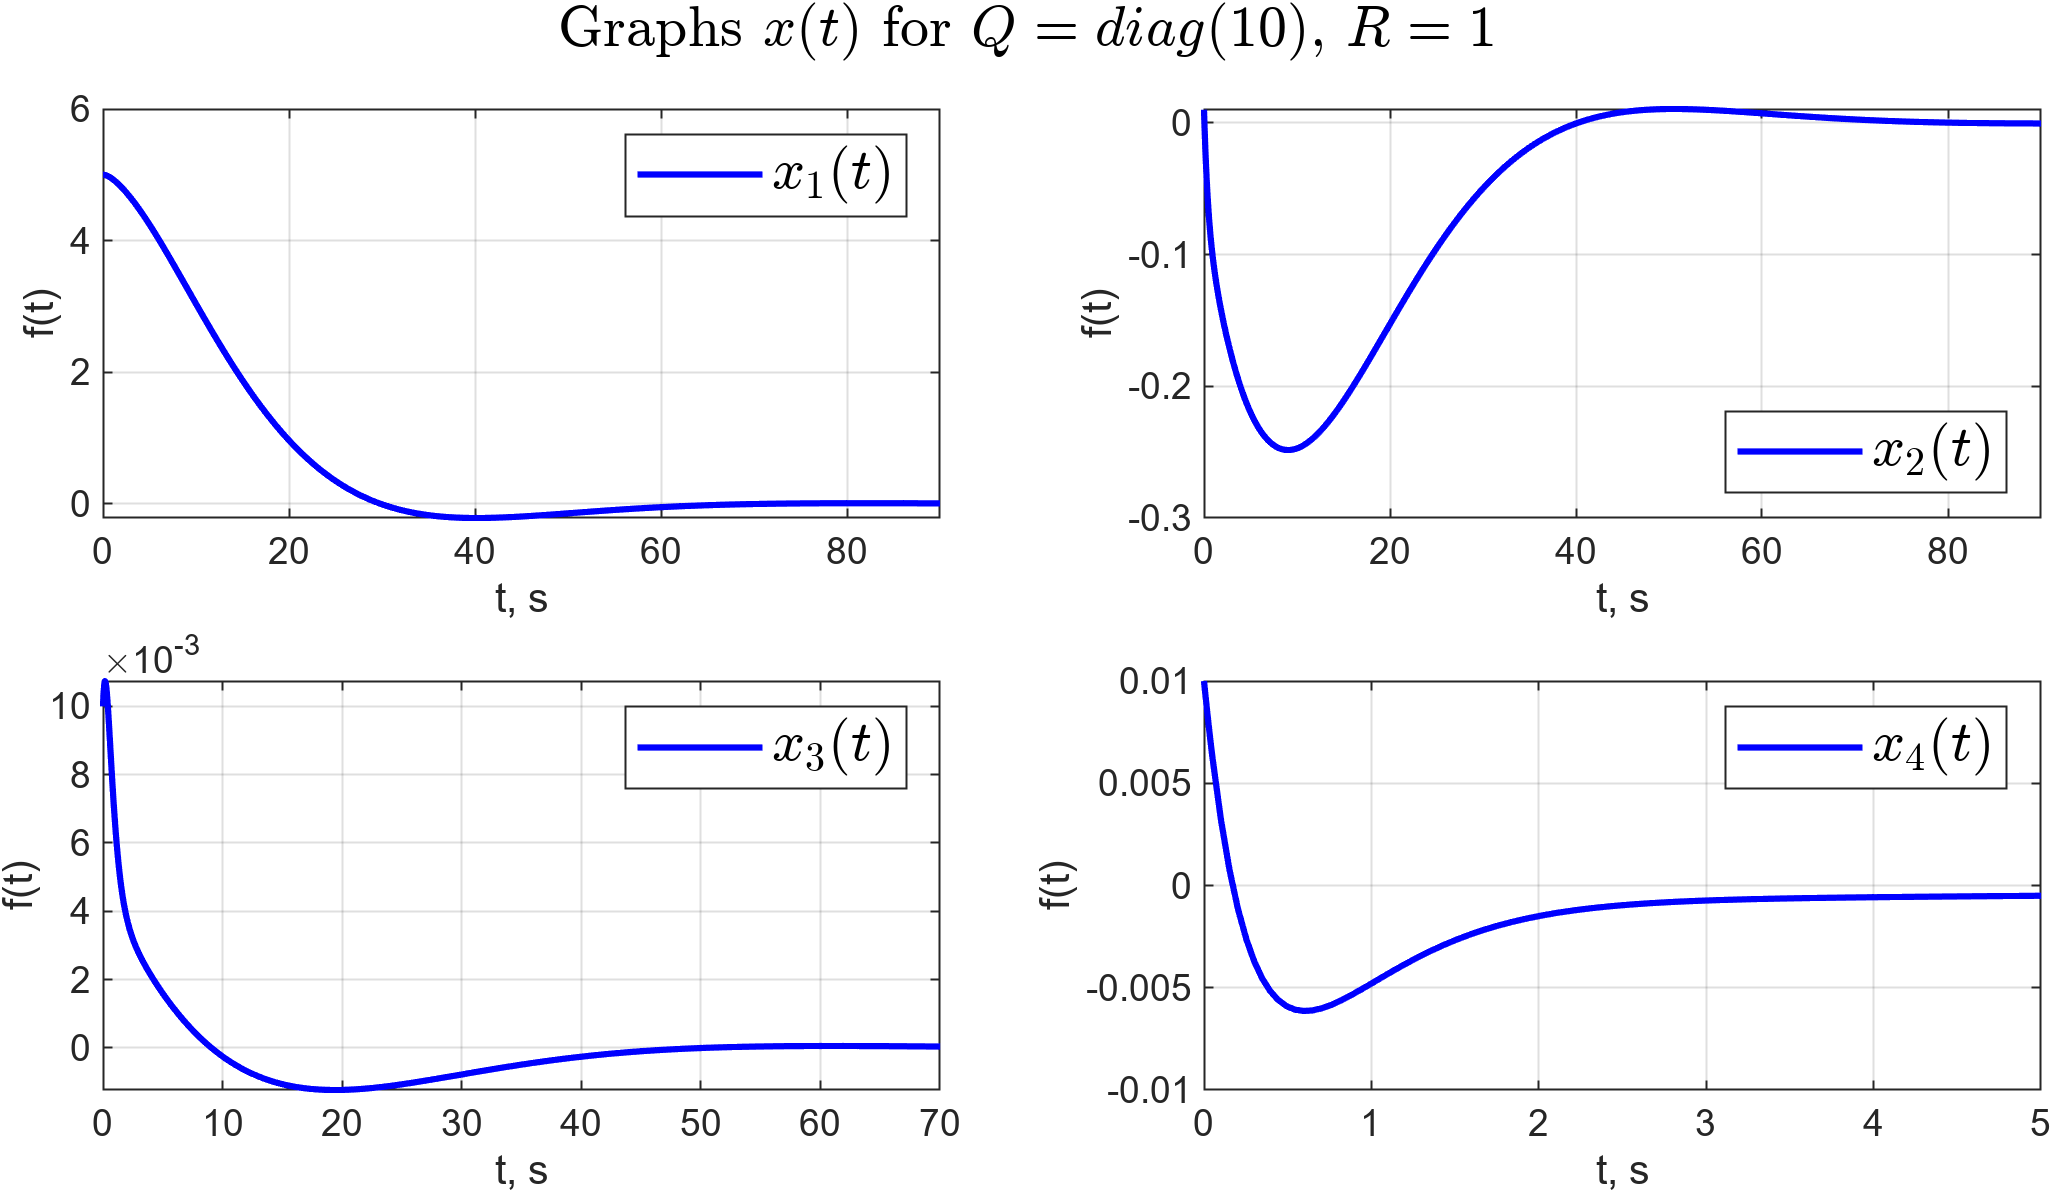
\includegraphics[width=1\linewidth]{pic2/6_lqr_n4.png}}
	\caption{Графики $x(t)$ для нелинейной системы при $x(0)=[5, \, \, 0.01, \, \, 0.01, \, \, 1.5]$.}
	\label{6_lqr_n4}
\end{figure}

\newpage
\,
\newpage
Для рассмотренных начальных условий синтезированный регулятор справляется с задачей стабилизации. Кроме того, амплитуда компонент вектора состояния минимальна (рисунки \ref{6_lqr_n1}, \ref{6_lqr_n2}, \ref{6_lqr_n3}, \ref{6_lqr_n4}).

\section{Исследование линейно-квадратичного регулятора}

Исследуем влияние весовых матриц LQR-регулятора на маскимальное отклонение маятника от вертикали, максимальное горизонтальное смещение тележки и максимальное значение управляющего сигнала при управлении нелинейной системой. Результаты представим в виде таблицы \ref{6_tab_1}, моделирование -- на рисунках \ref{6_2_Q_1_R_10_x}-\ref{6_2_Q_1_R_1_u} (компоненты вектора состояния системы $x(t)$ в данном случае обозначены через соответствующие физические величины).

\begin{table}[h]
	\centering
	\caption{Результаты моделирования при разных значениях весовых матриц.}
	\label{6_tab_1}
	\begin{tabular}{ccccc}
		\toprule
		$Q$, diag & $R$ & $\max |\varphi|$ & $\max |a|$ & $\max |u|$ \\
		\midrule
		1  & 10  &  0.01  &  1.43  &  77  \\
		10  & 10 &  0.01  &  0.81  &  78  \\
		25 & 10&  0.01  &  0.65  &  79  \\
		50  &10&   0.01  &  0.55&  80 \\
		50  &1&   0.01  &  0.32 &  83  \\
		25  &1&   0.01  &  0.37 &  82  \\
		1  &1&   0.01  &  0.81 &  78 \\
		\bottomrule
	\end{tabular}
\end{table}

% Q=1 R=10
\begin{figure}[!h]
	\center{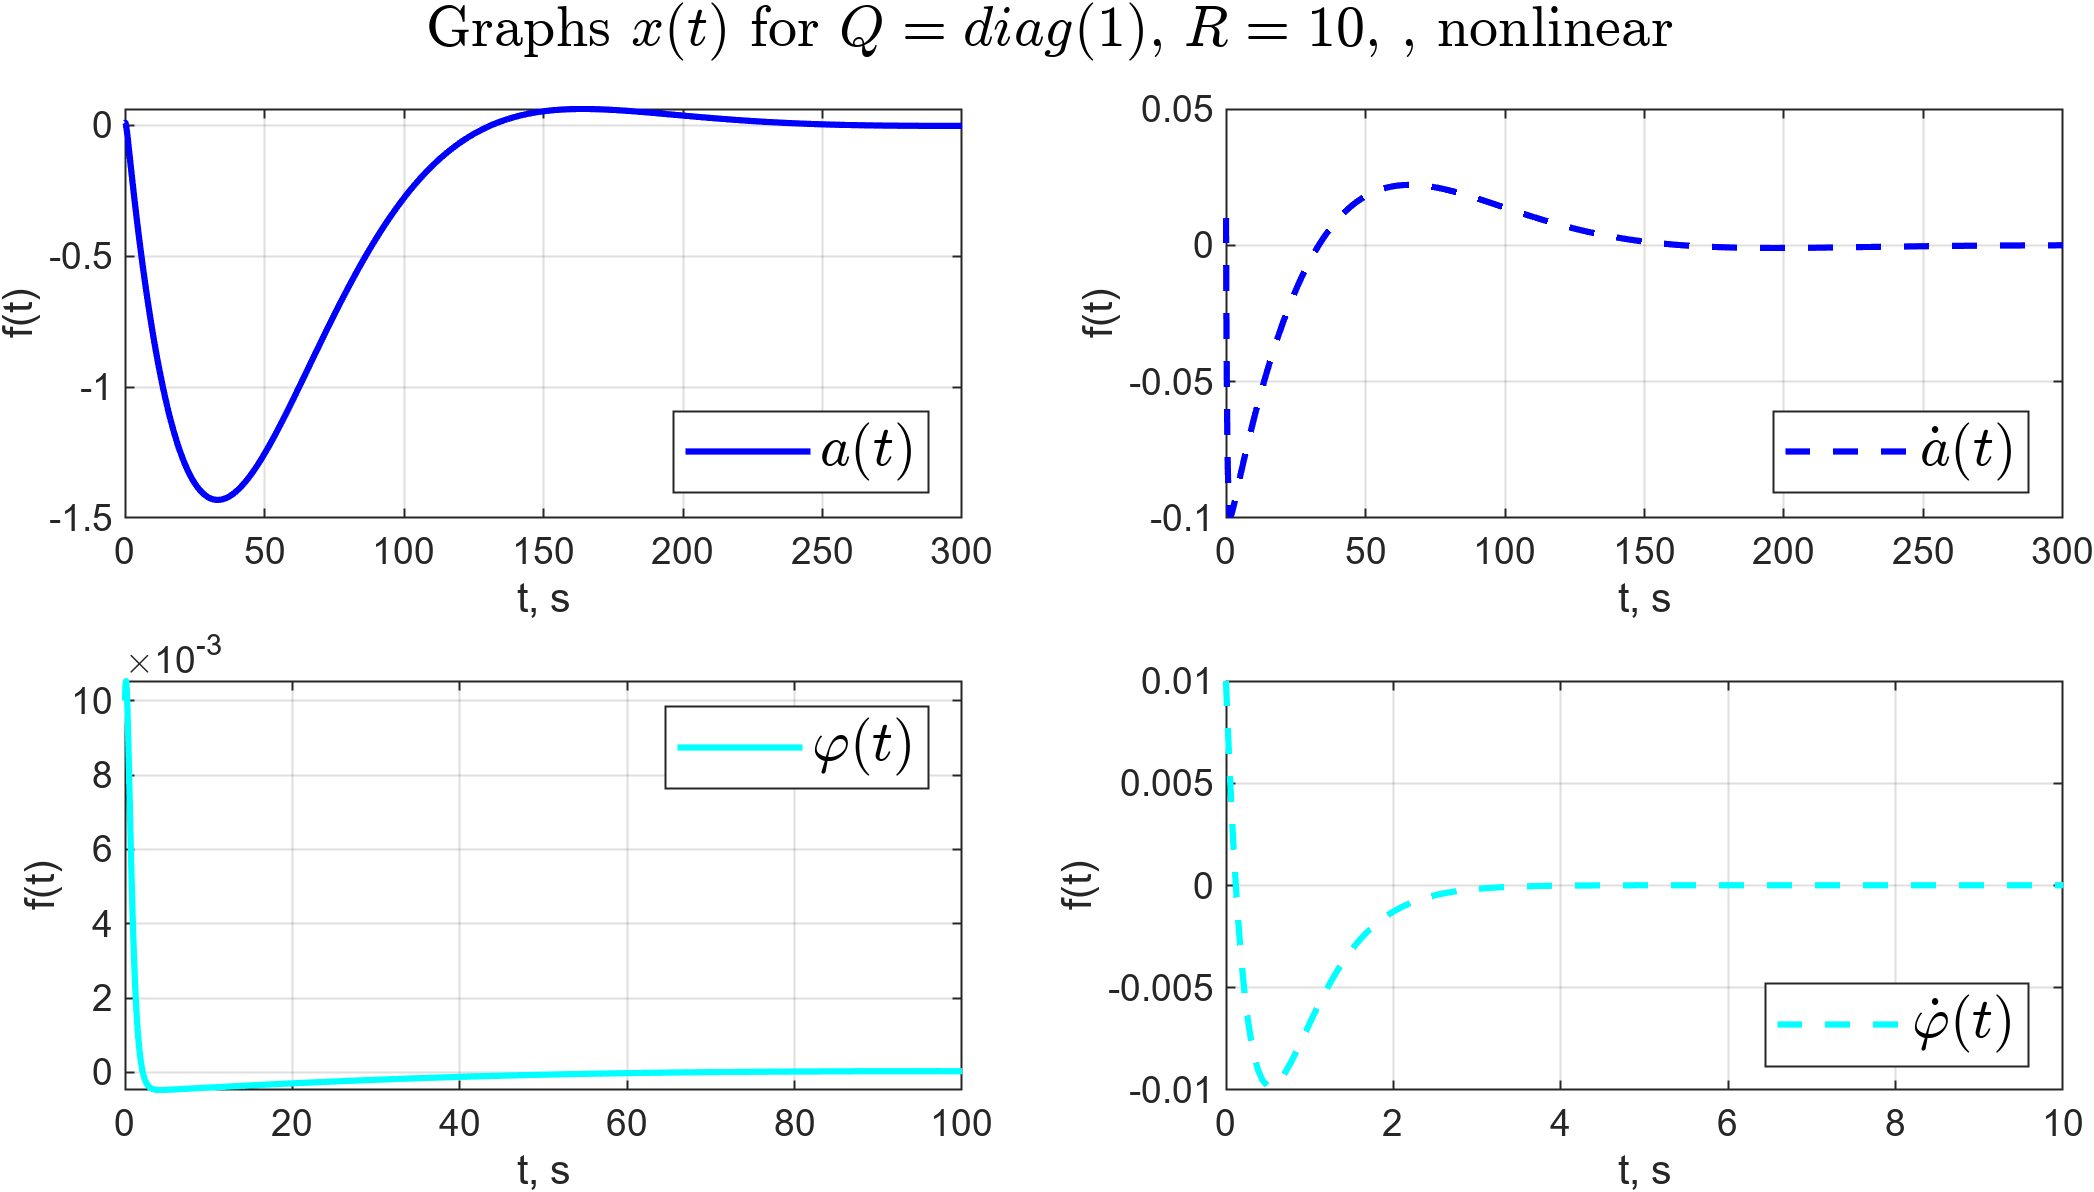
\includegraphics[width=1\linewidth]{pic_fix/6_2_Q_1_R_10_x.png}}
	\caption{Графики компонент вектора состояния системы при $Q=diag(1)$, $R=10$.}
	\label{6_2_Q_1_R_10_x}
\end{figure}

\begin{figure}[!h]
	\center{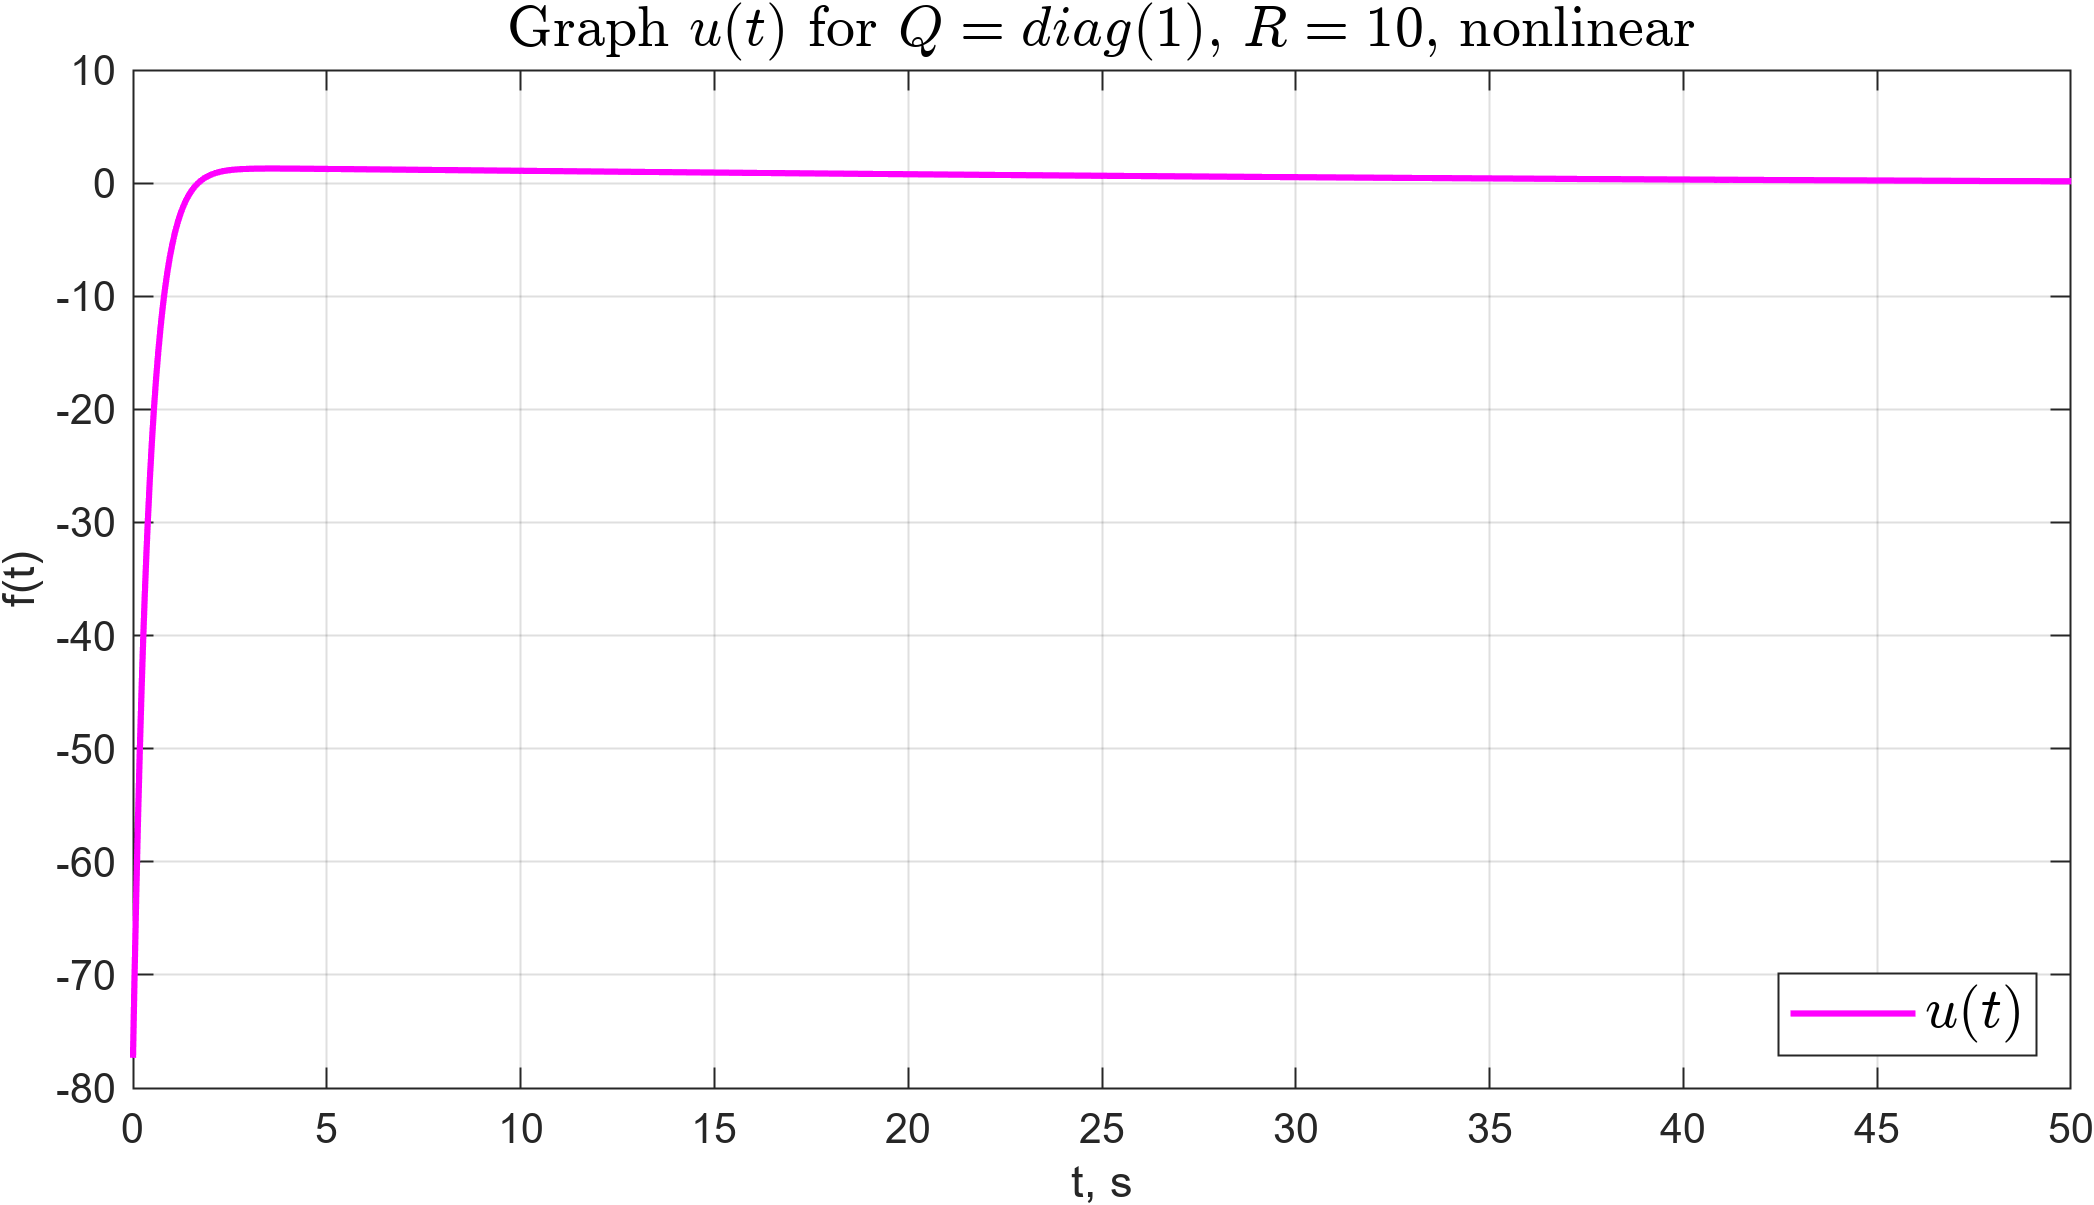
\includegraphics[width=1\linewidth]{pic_fix/6_2_Q_1_R_10_u.png}}
	\caption{График $u(t)$ при $Q=diag(1)$, $R=10$.}
	\label{6_2_Q_1_R_10_u}
\end{figure}

% Q=10 R=10
\begin{figure}[!h]
	\center{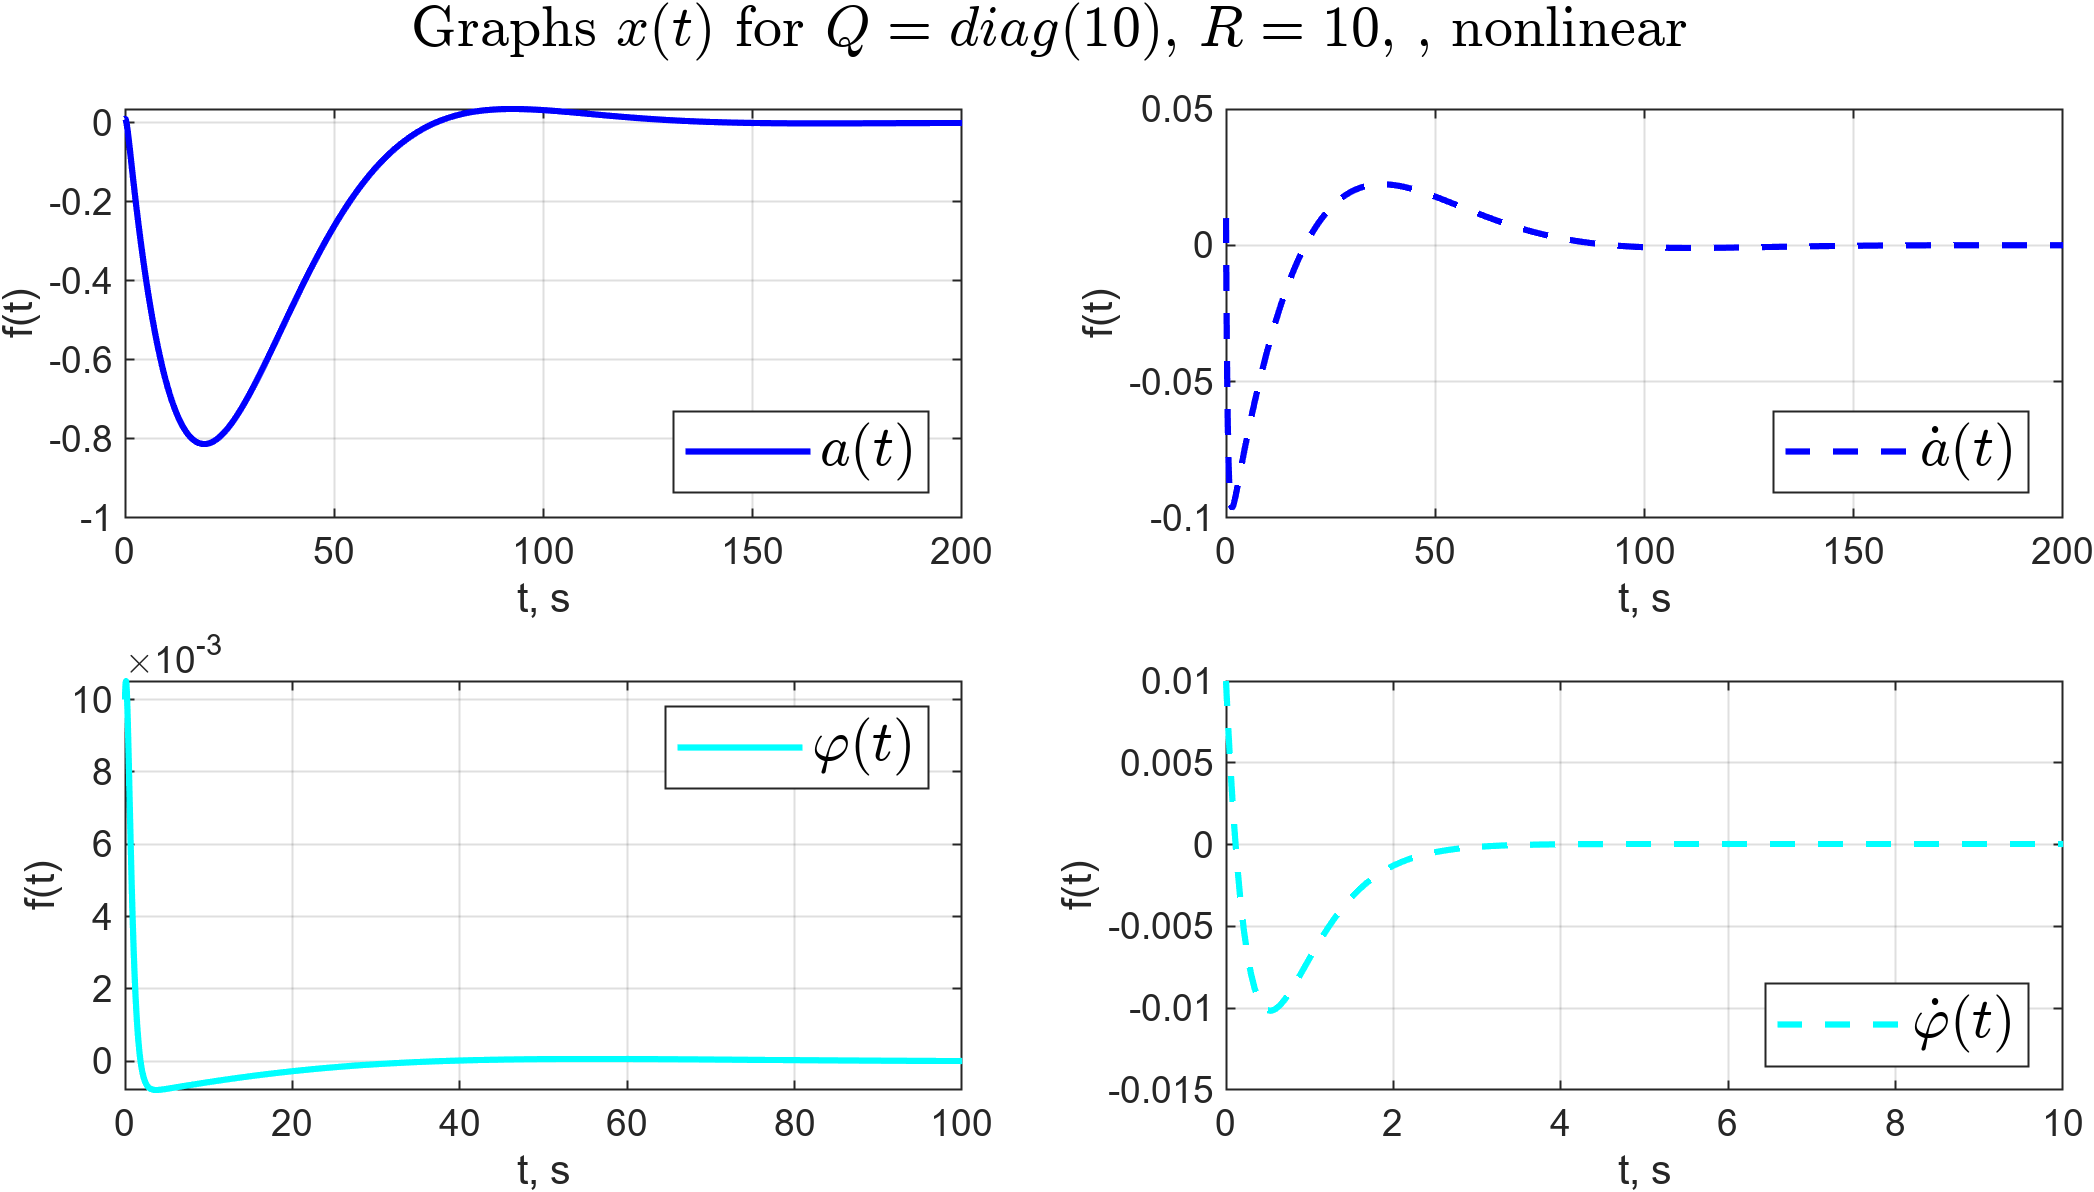
\includegraphics[width=1\linewidth]{pic_fix/6_2_Q_10_R_10_x.png}}
	\caption{Графики компонент вектора состояния системы при $Q=diag(10)$, $R=10$.}
	\label{6_2_Q_10_R_10_x}
\end{figure}

\begin{figure}[!h]
	\center{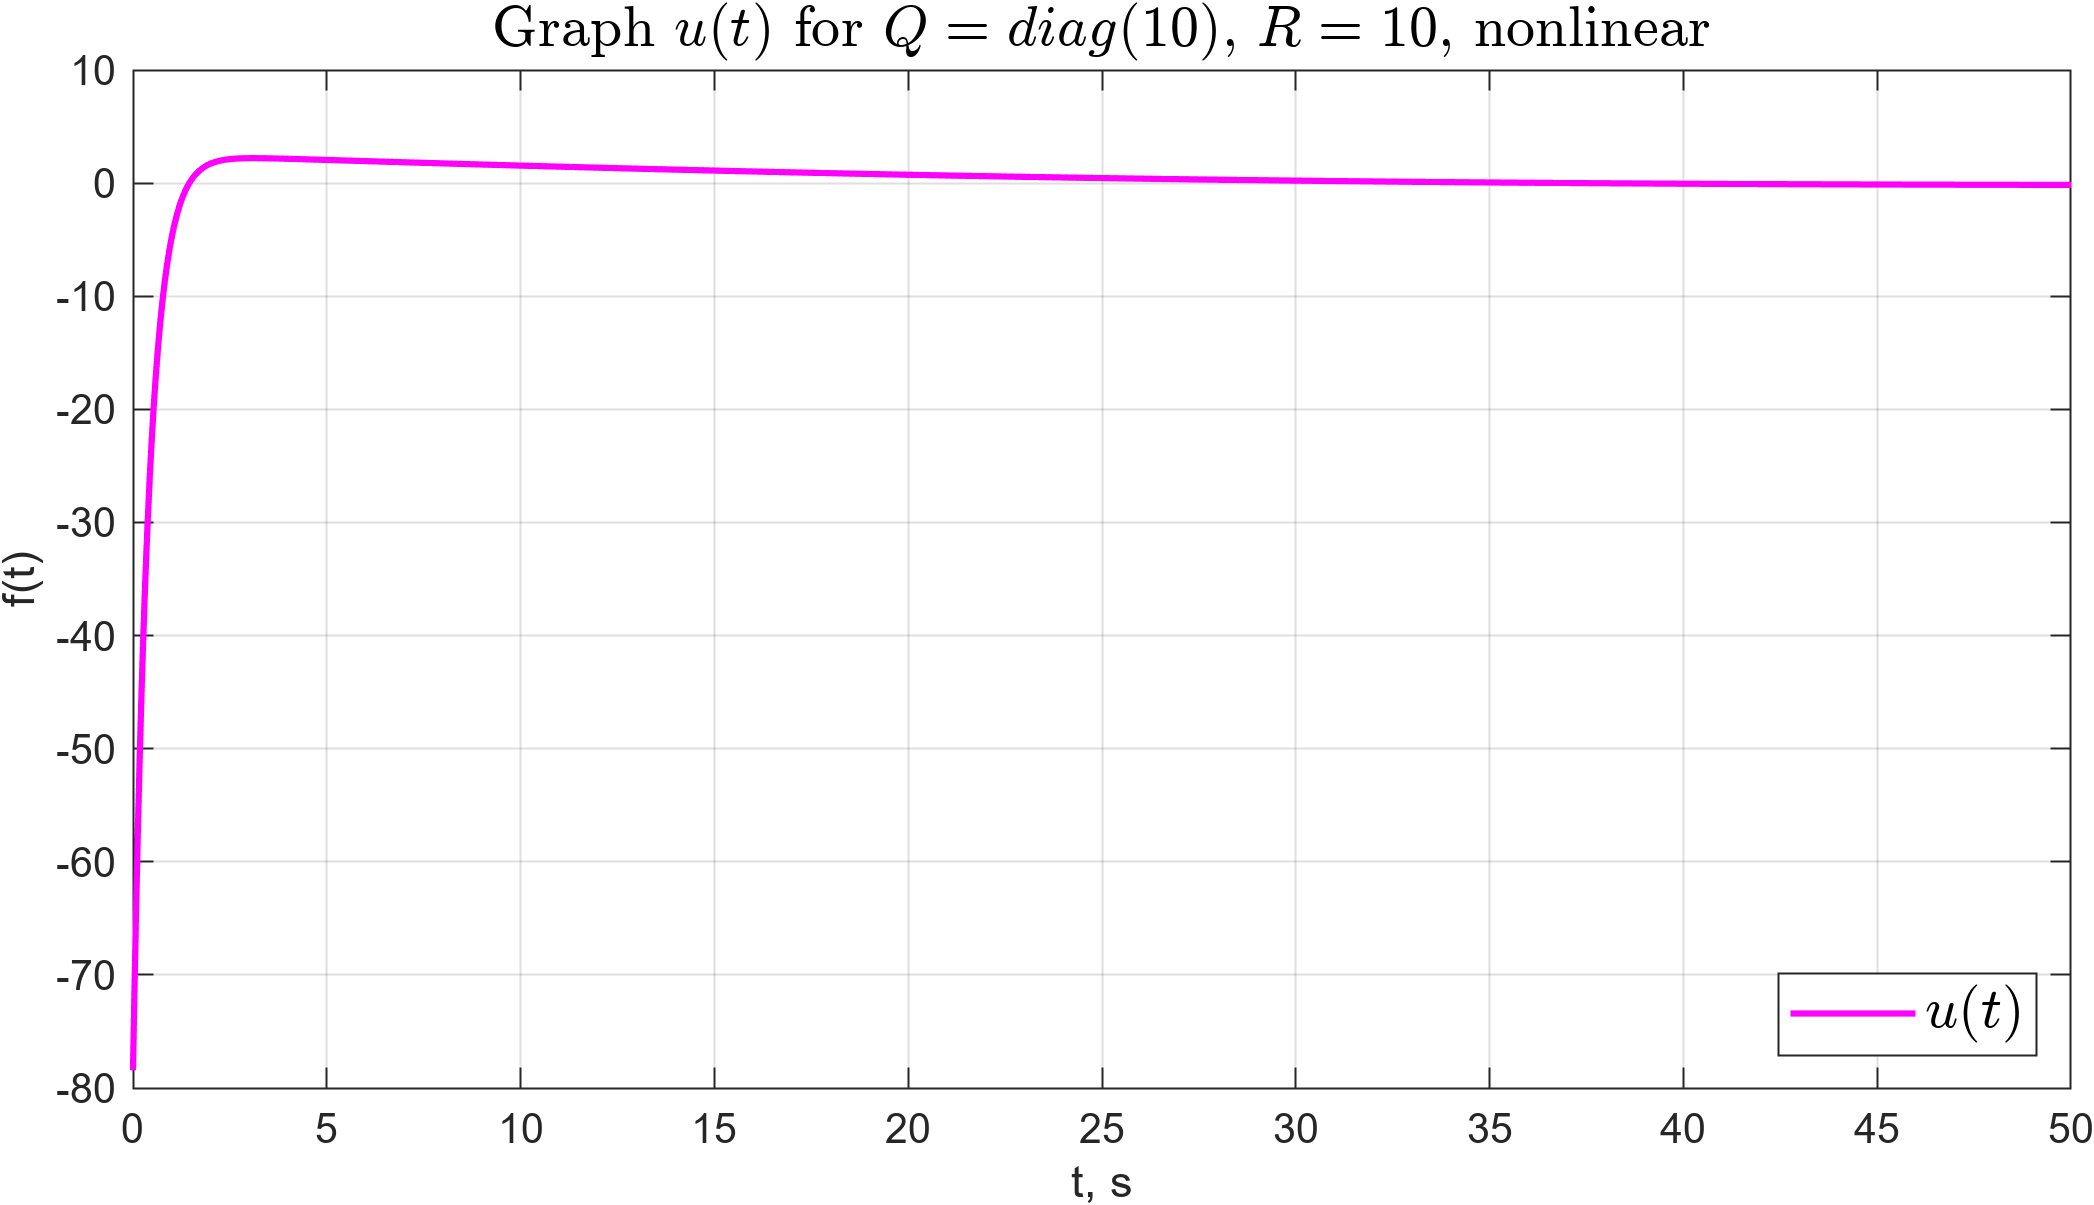
\includegraphics[width=1\linewidth]{pic_fix/6_2_Q_10_R_10_u.png}}
	\caption{График $u(t)$ при $Q=diag(10)$, $R=10$.}
	\label{6_2_Q_10_R_10_u}
\end{figure}

% Q=25 R=10
\begin{figure}[!h]
	\center{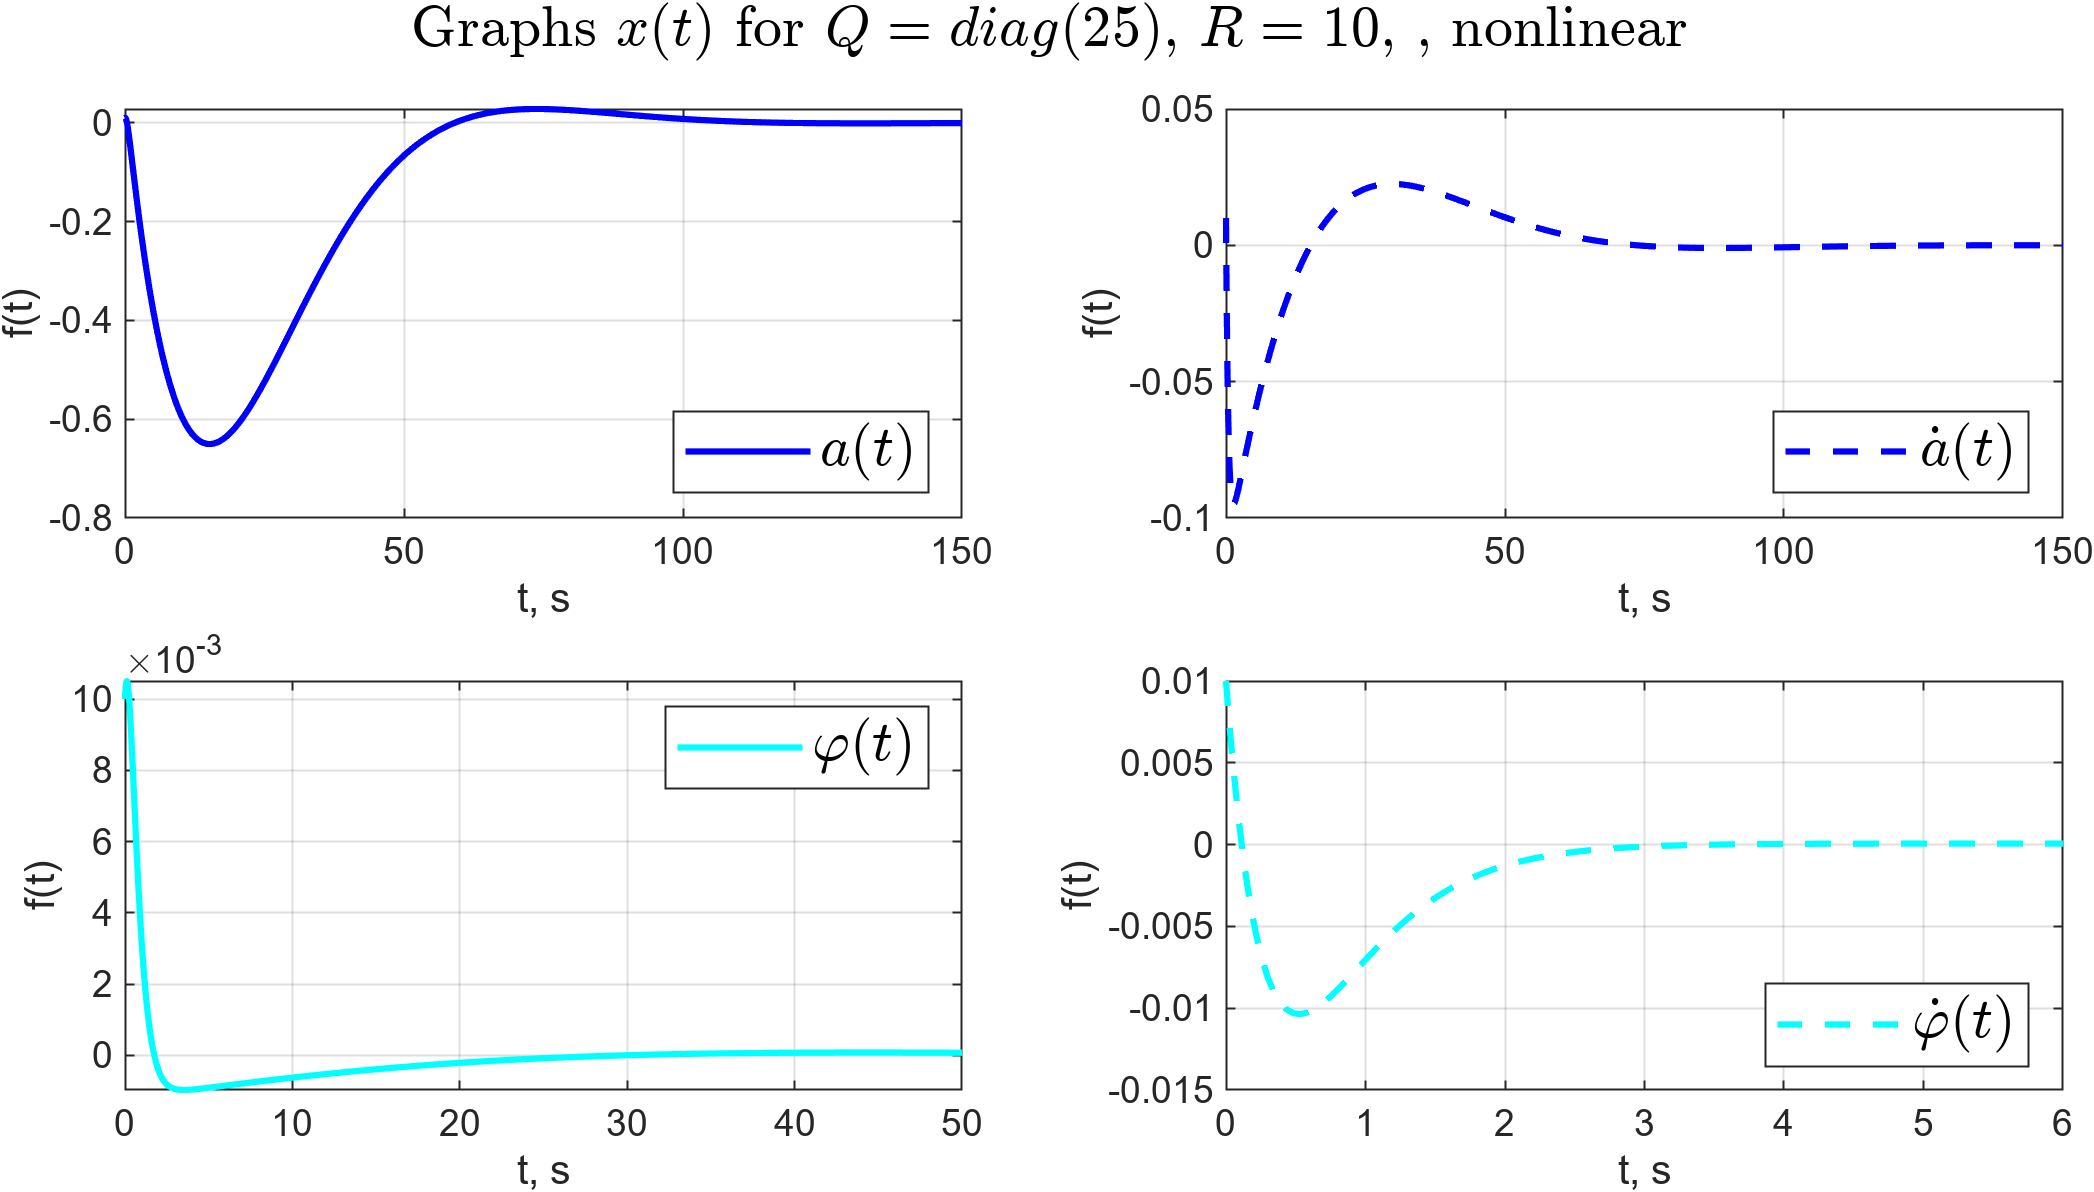
\includegraphics[width=1\linewidth]{pic_fix/6_2_Q_25_R_10_x.png}}
	\caption{Графики компонент вектора состояния системы при $Q=diag(25)$, $R=10$.}
	\label{6_2_Q_25_R_10_x}
\end{figure}

\begin{figure}[!h]
	\center{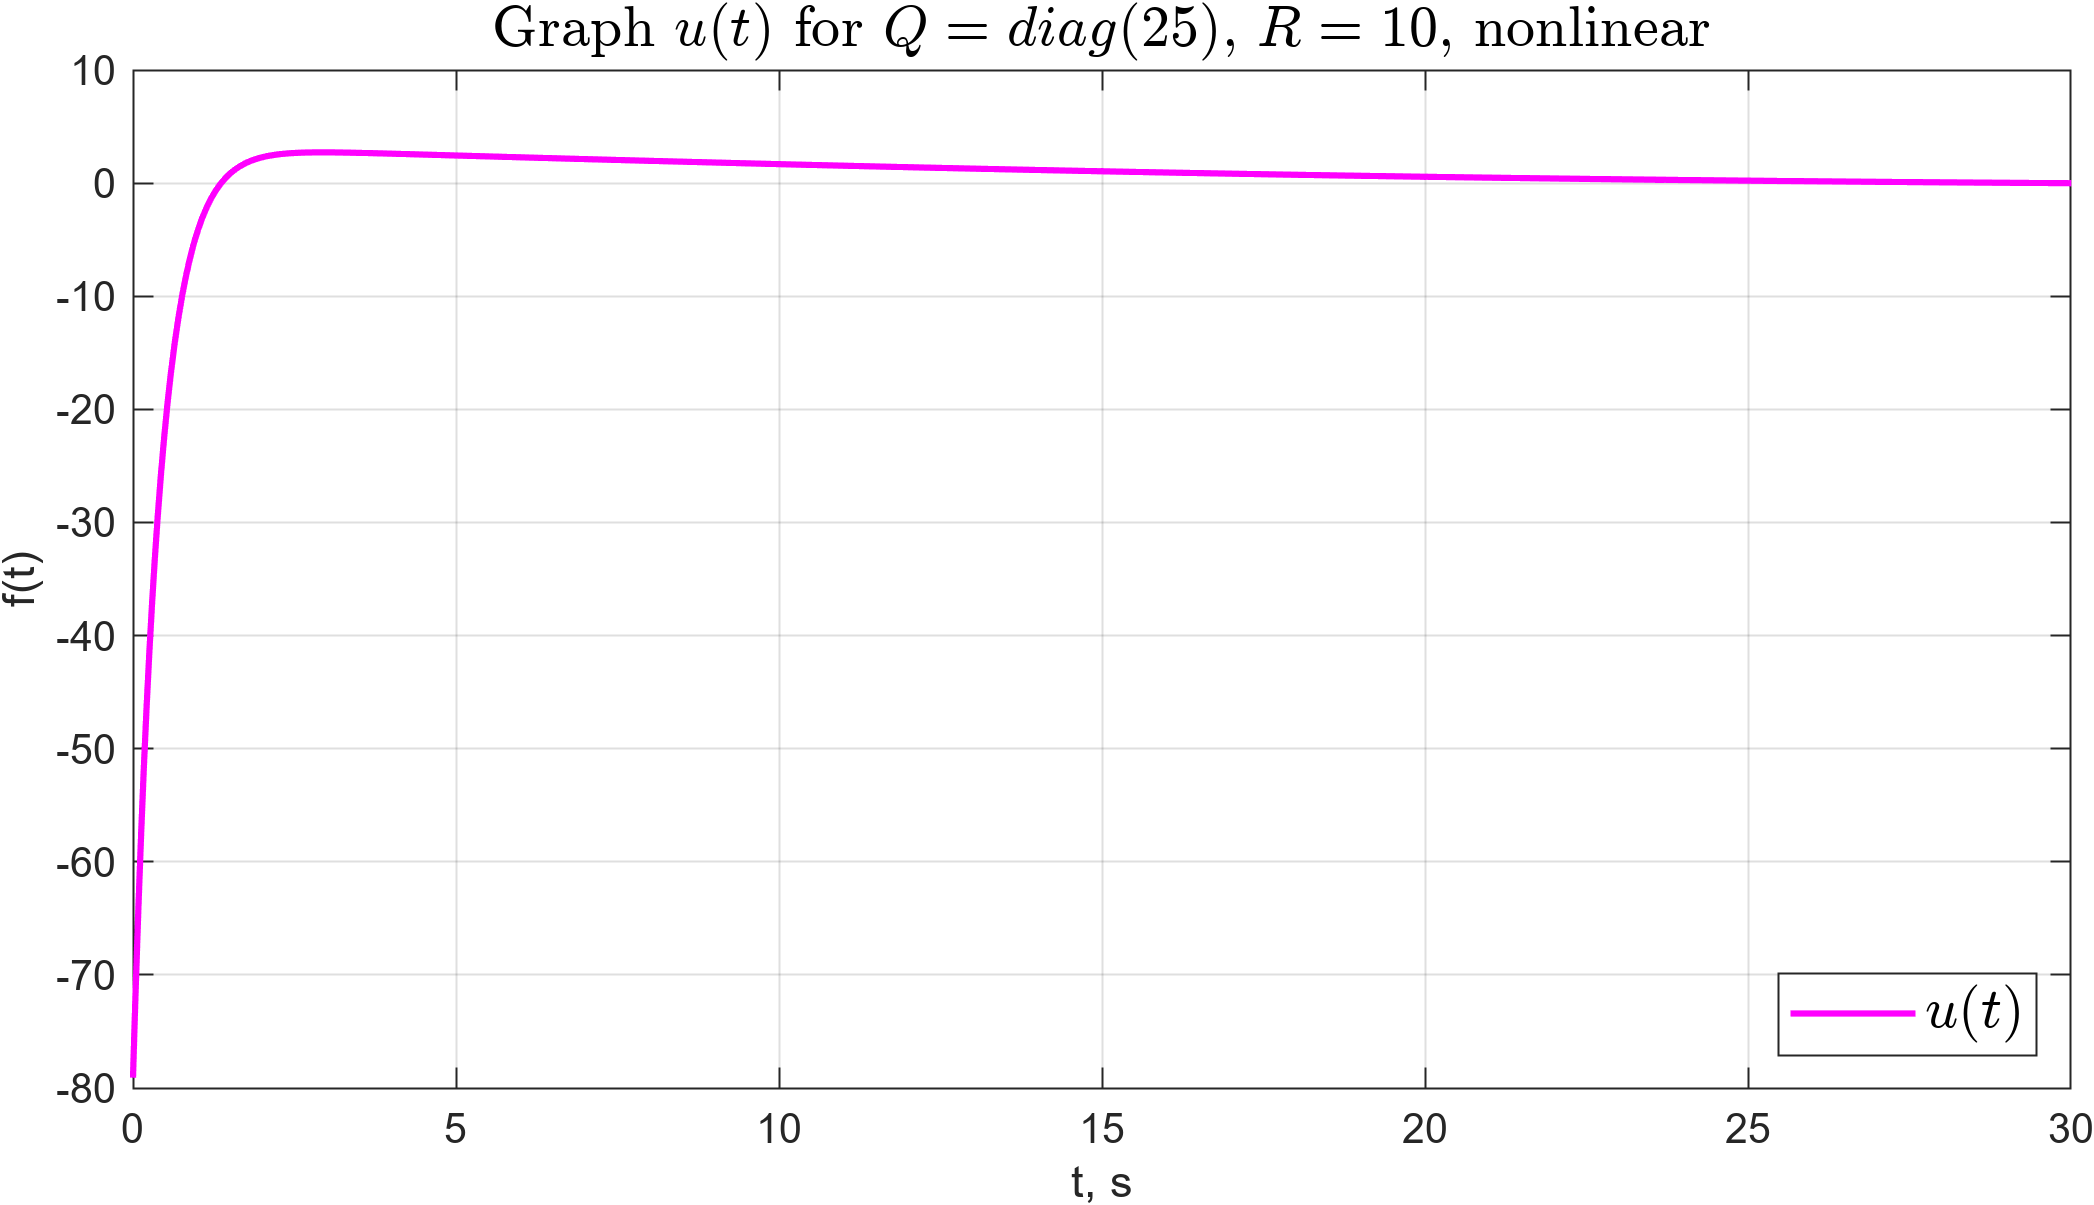
\includegraphics[width=1\linewidth]{pic_fix/6_2_Q_25_R_10_u.png}}
	\caption{График $u(t)$ при $Q=diag(25)$, $R=10$.}
	\label{6_2_Q_25_R_10_u}
\end{figure}


% Q=50 R=10
\begin{figure}[!h]
	\center{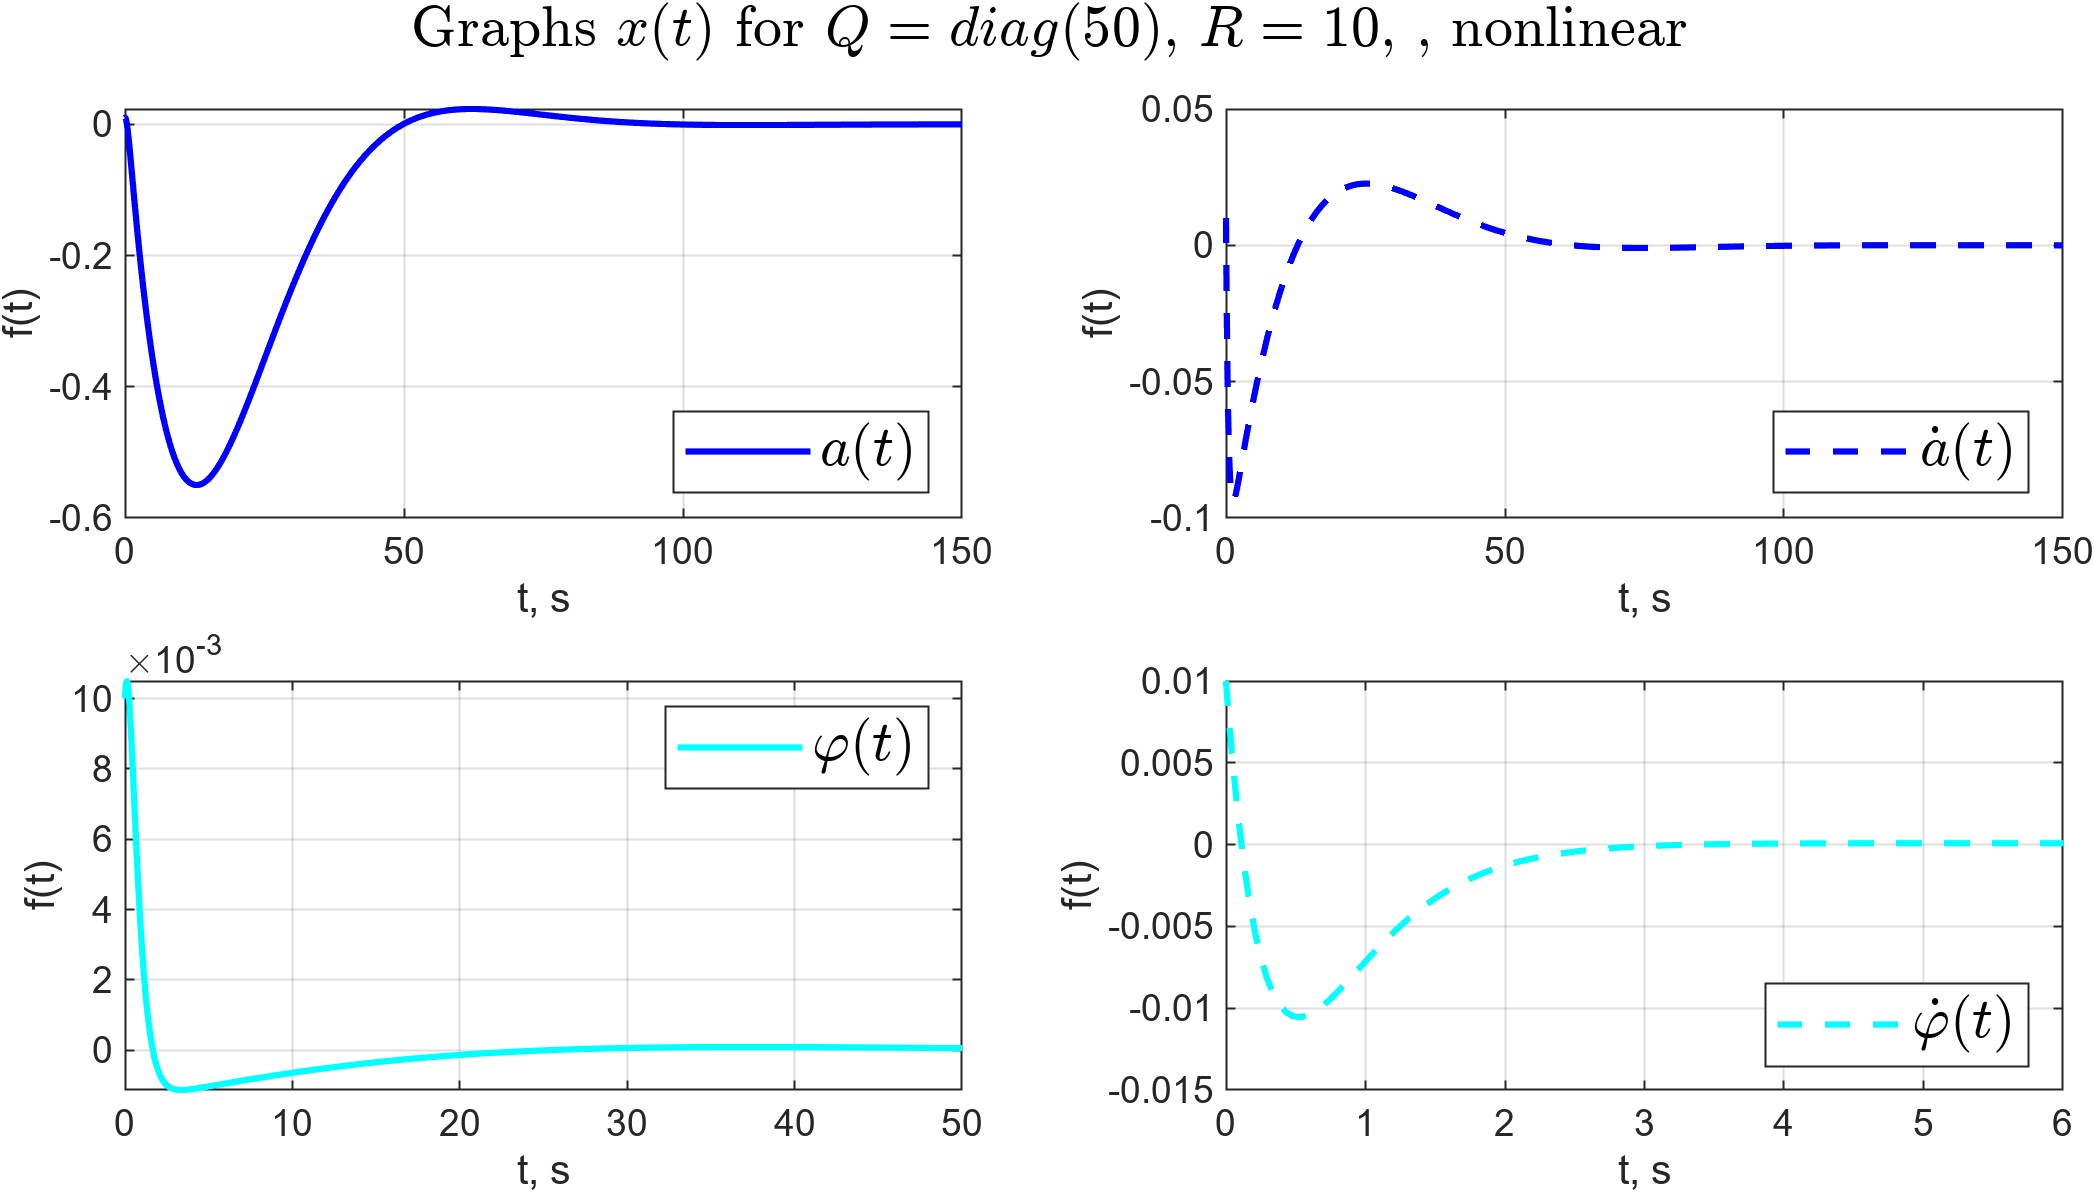
\includegraphics[width=1\linewidth]{pic_fix/6_2_Q_50_R_10_x.png}}
	\caption{Графики компонент вектора состояния системы при $Q=diag(50)$, $R=10$.}
	\label{6_2_Q_50_R_10_x}
\end{figure}

\begin{figure}[!h]
	\center{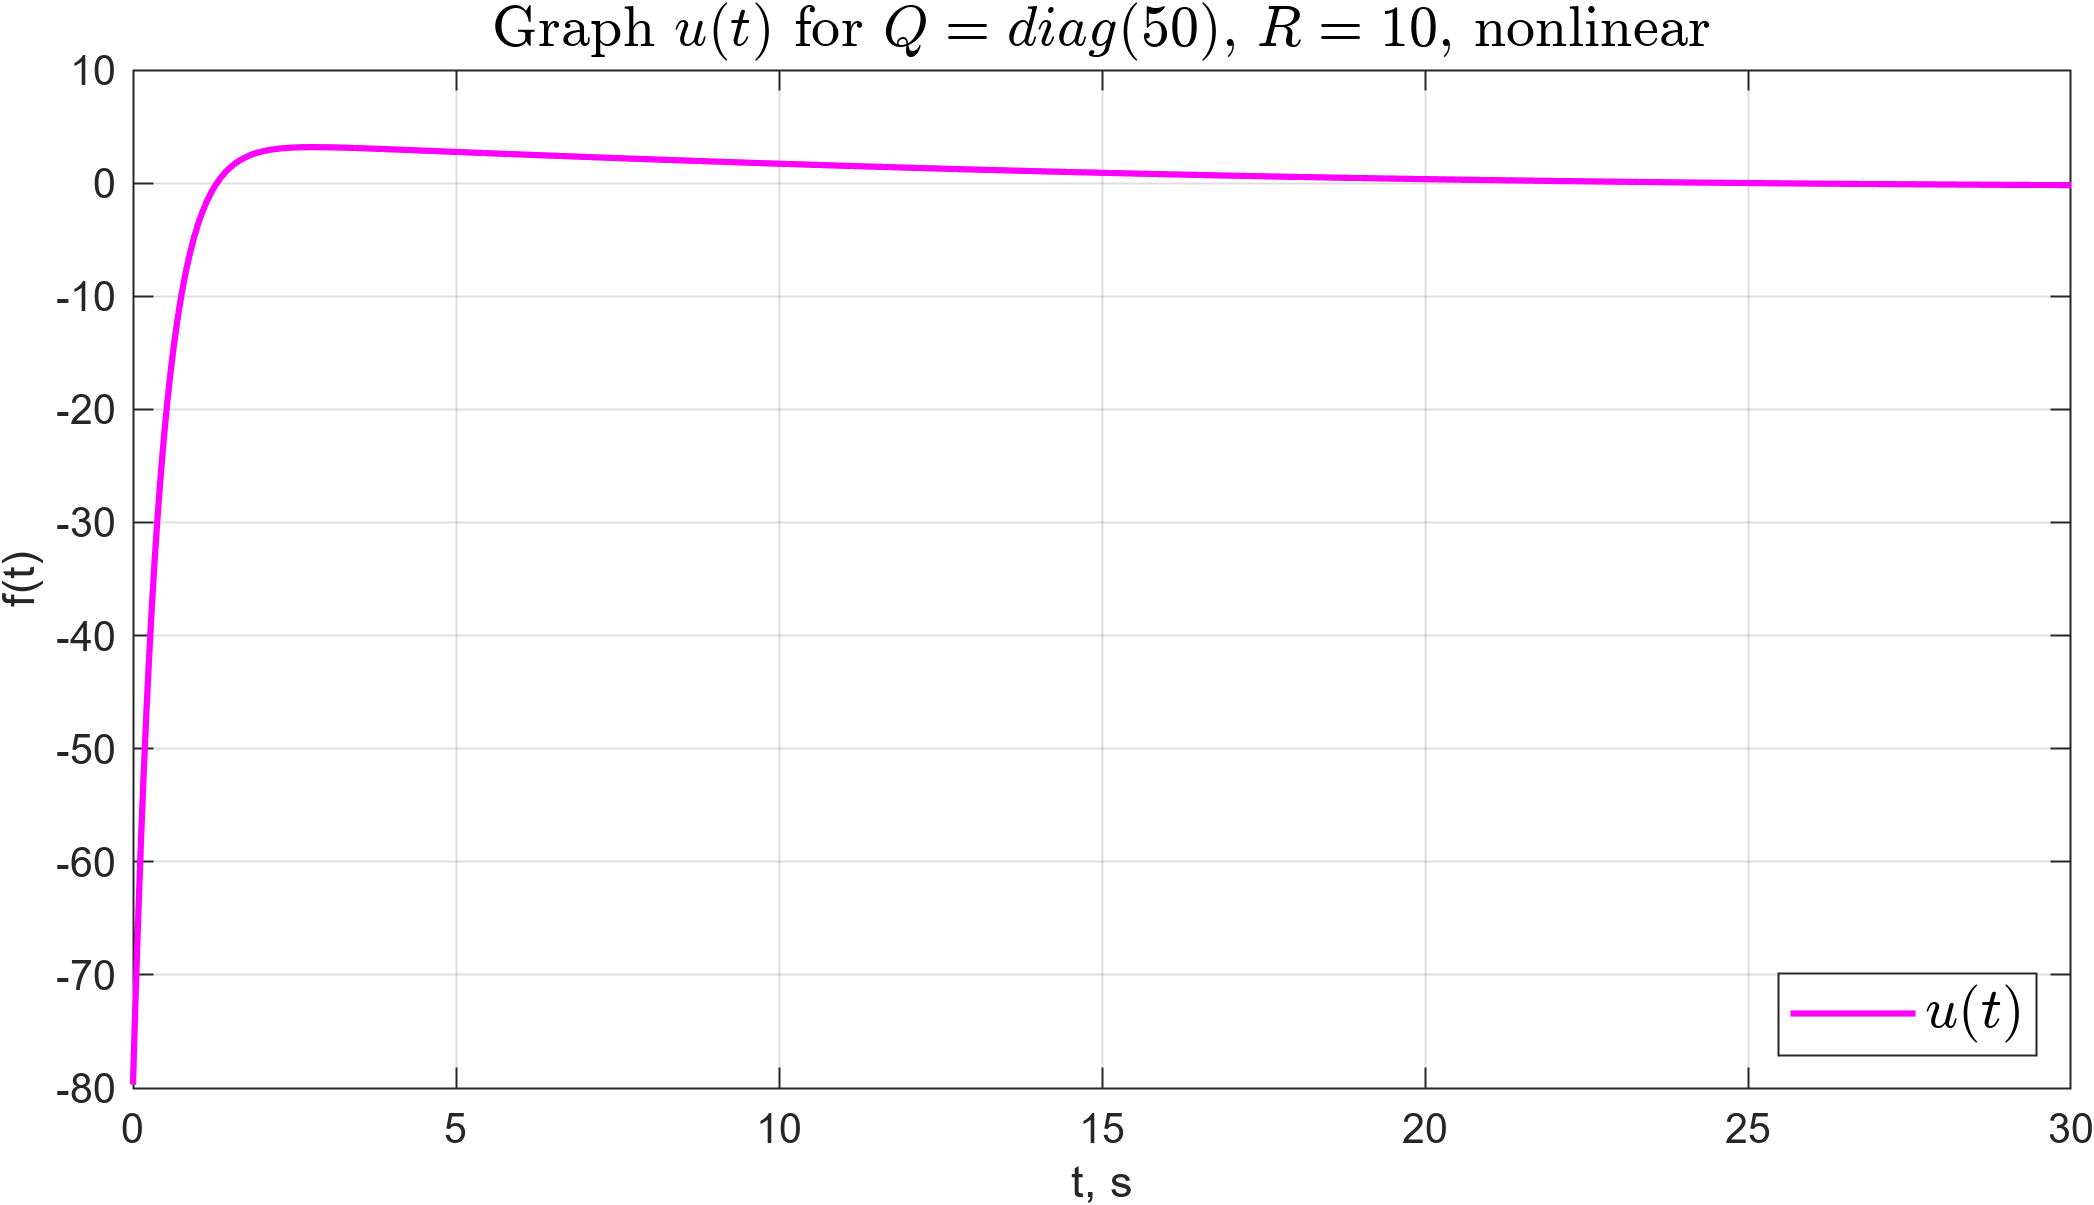
\includegraphics[width=1\linewidth]{pic_fix/6_2_Q_50_R_10_u.png}}
	\caption{График $u(t)$ при $Q=diag(50)$, $R=10$.}
	\label{6_2_Q_50_R_10_u}
\end{figure}

% Q=50 R=1
\begin{figure}[!h]
	\center{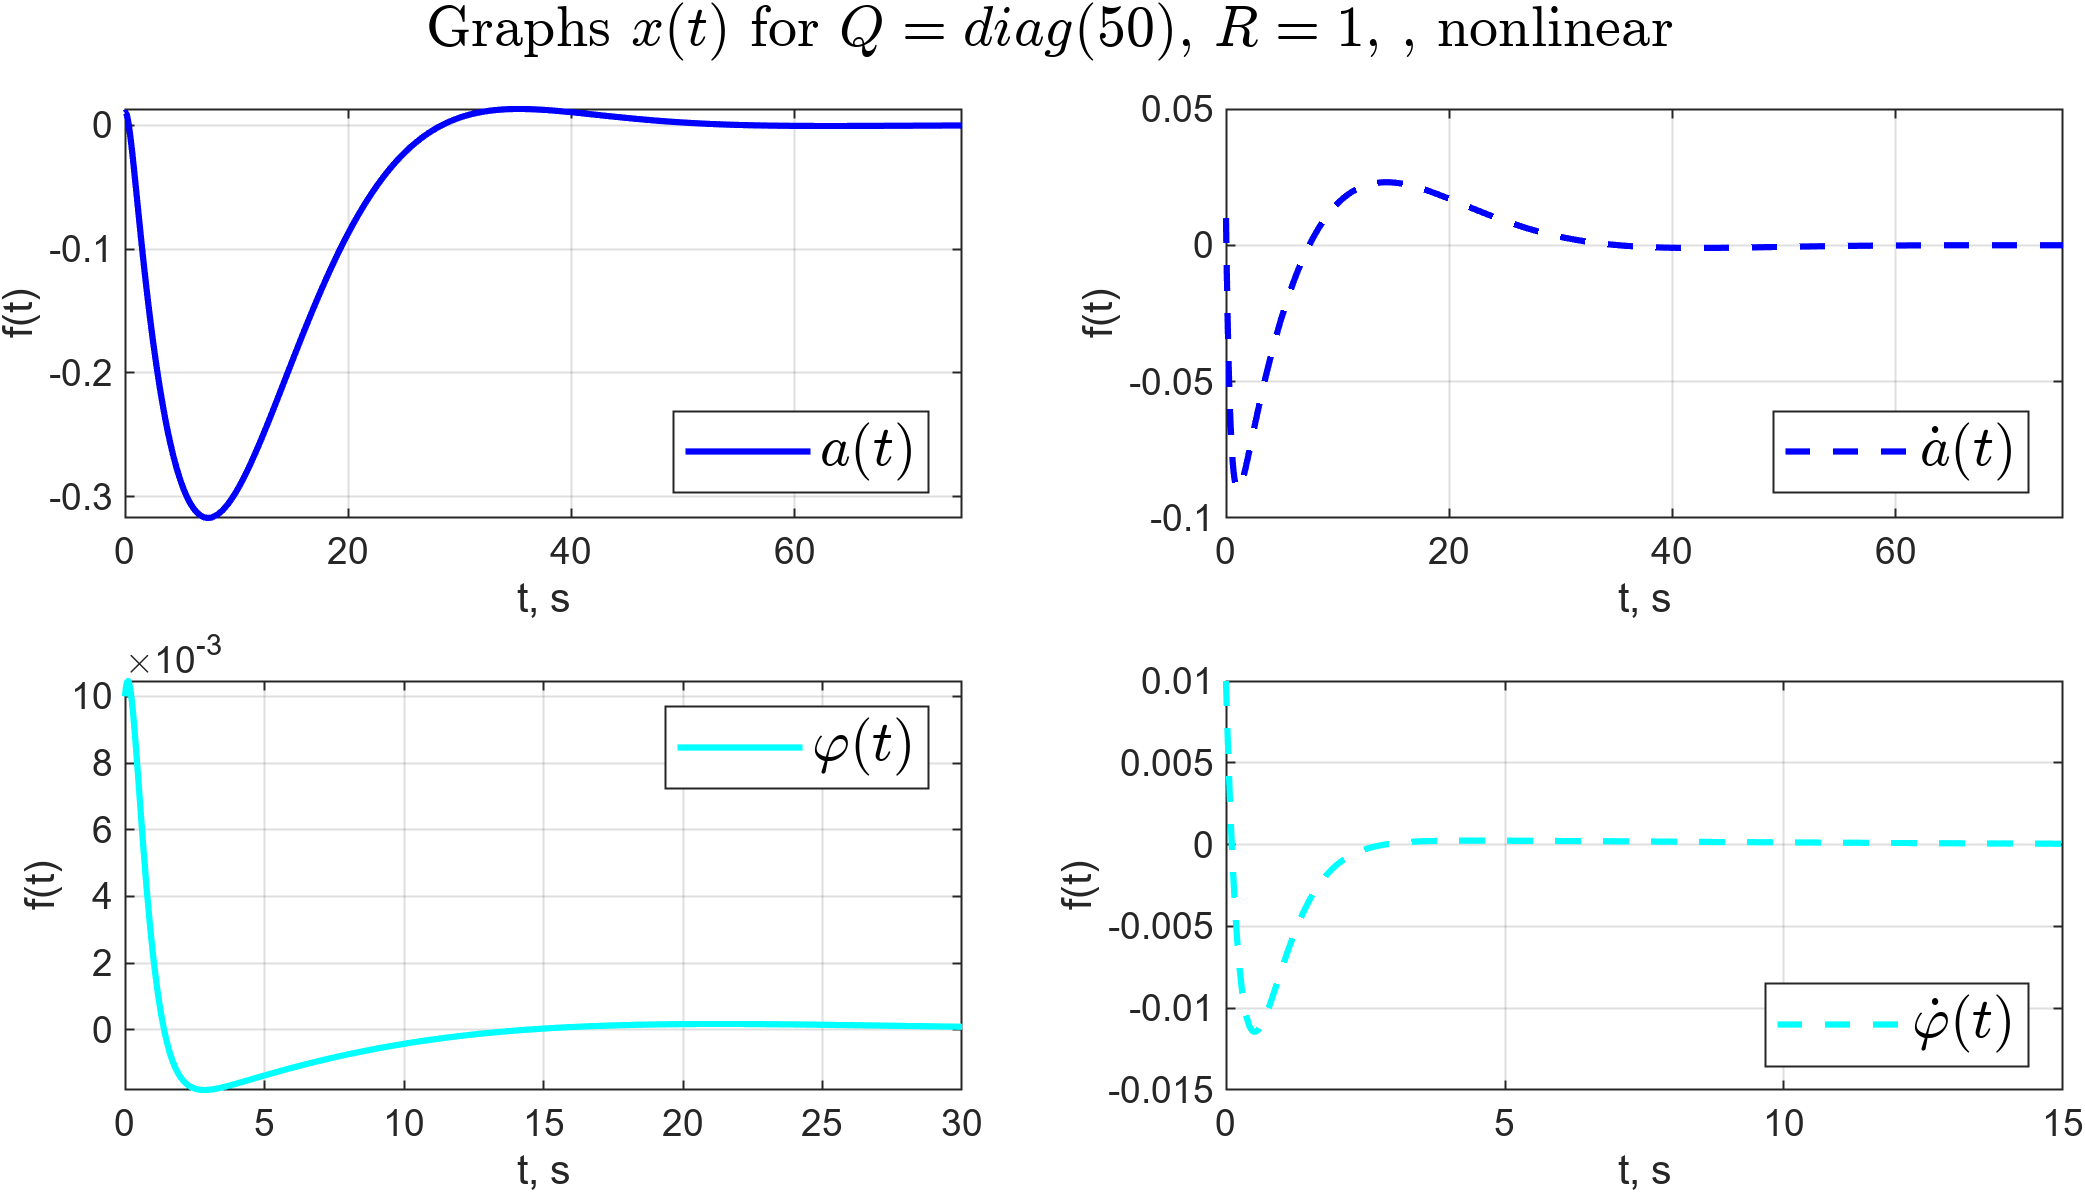
\includegraphics[width=1\linewidth]{pic_fix/6_2_Q_50_R_1_x.png}}
	\caption{Графики компонент вектора состояния системы при $Q=diag(50)$, $R=1$.}
	\label{6_2_Q_50_R_1_x}
\end{figure}

\begin{figure}[!h]
	\center{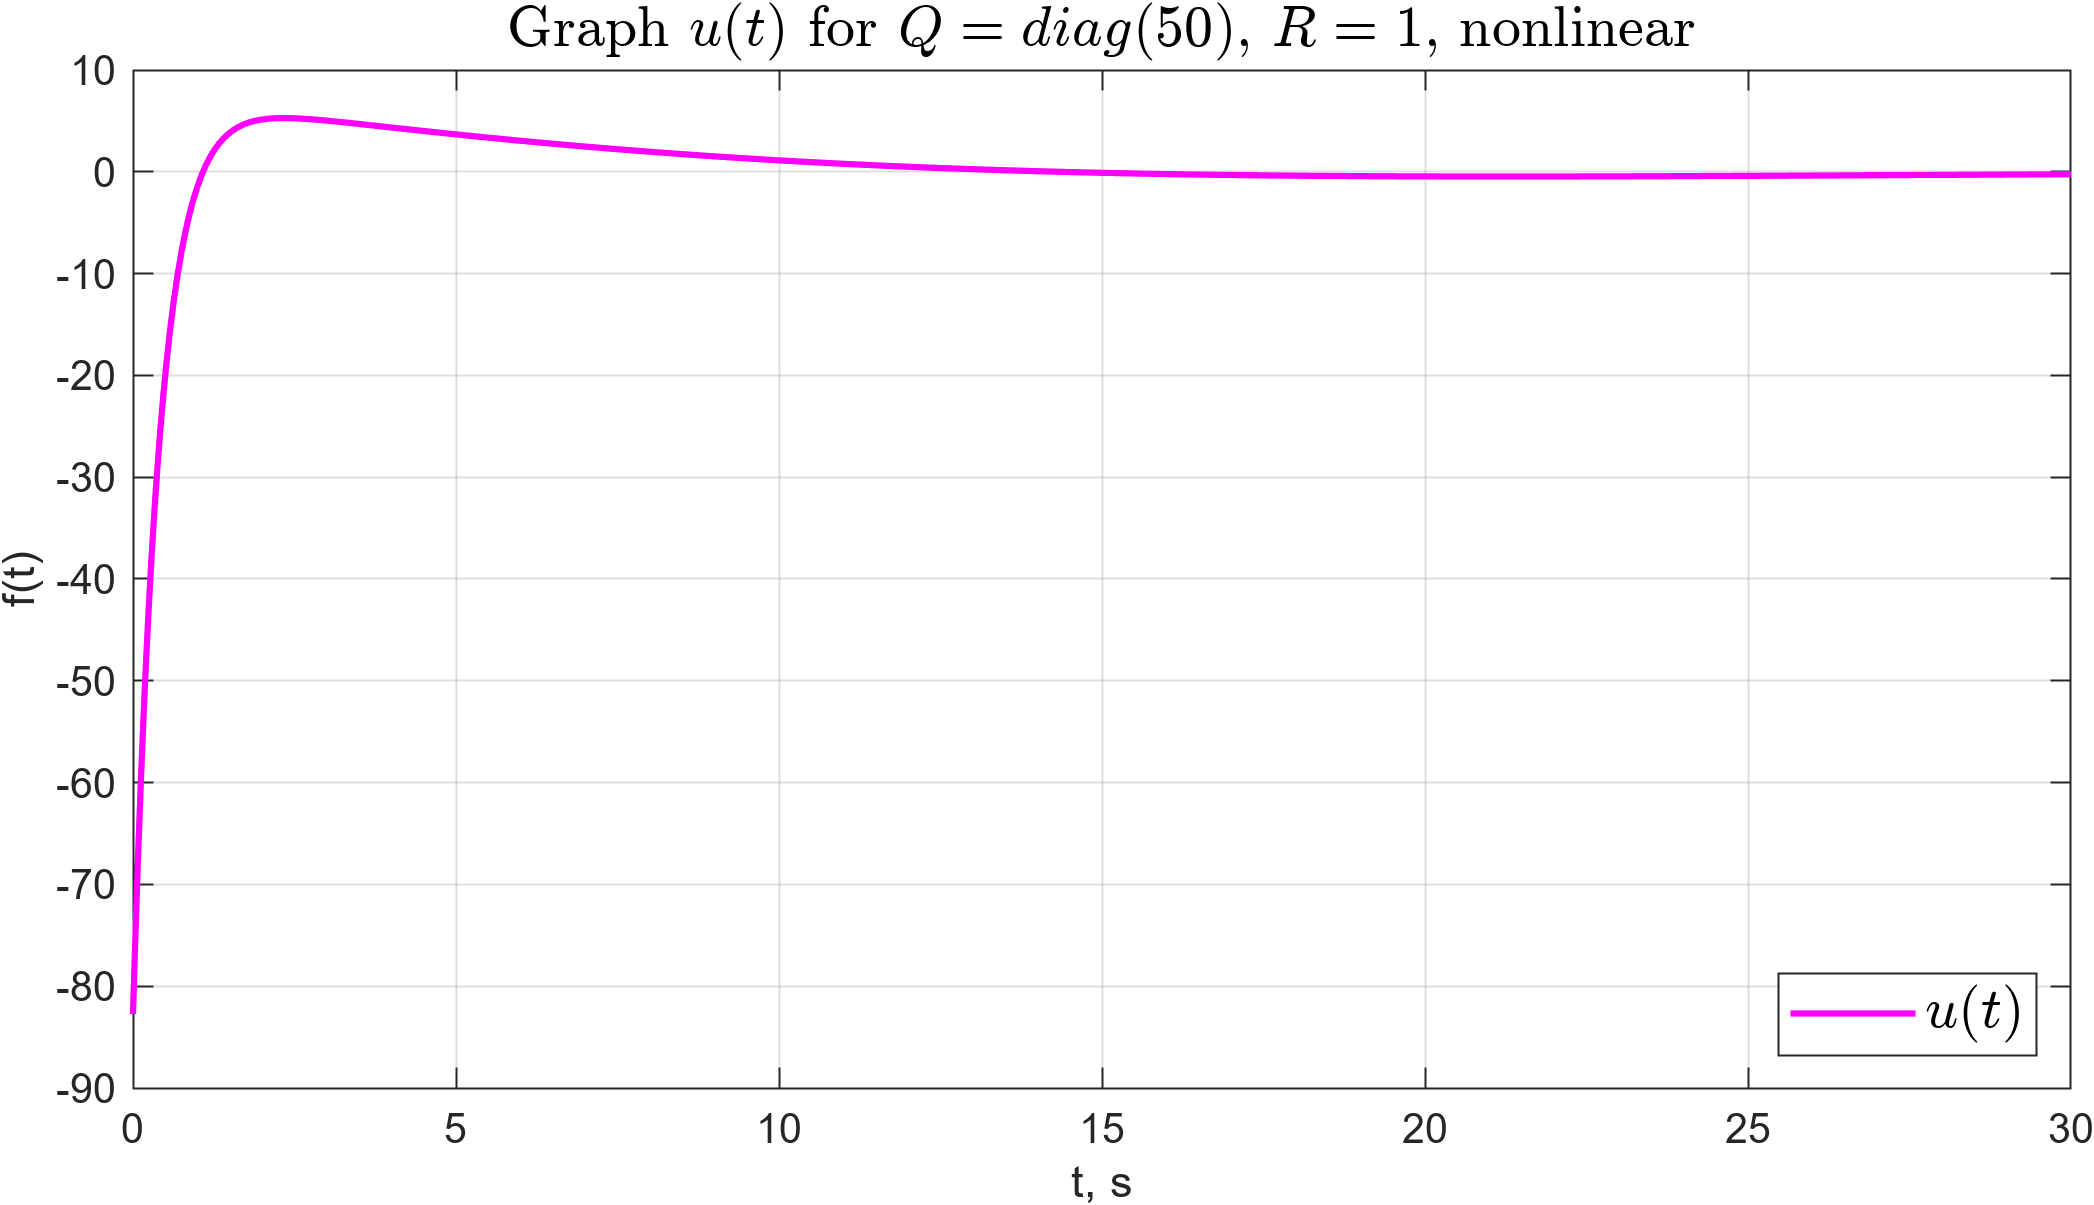
\includegraphics[width=1\linewidth]{pic_fix/6_2_Q_50_R_1_u.png}}
	\caption{График $u(t)$ при $Q=diag(50)$, $R=1$.}
	\label{6_2_Q_50_R_1_u}
\end{figure}


% Q=25 R=1
\begin{figure}[!h]
	\center{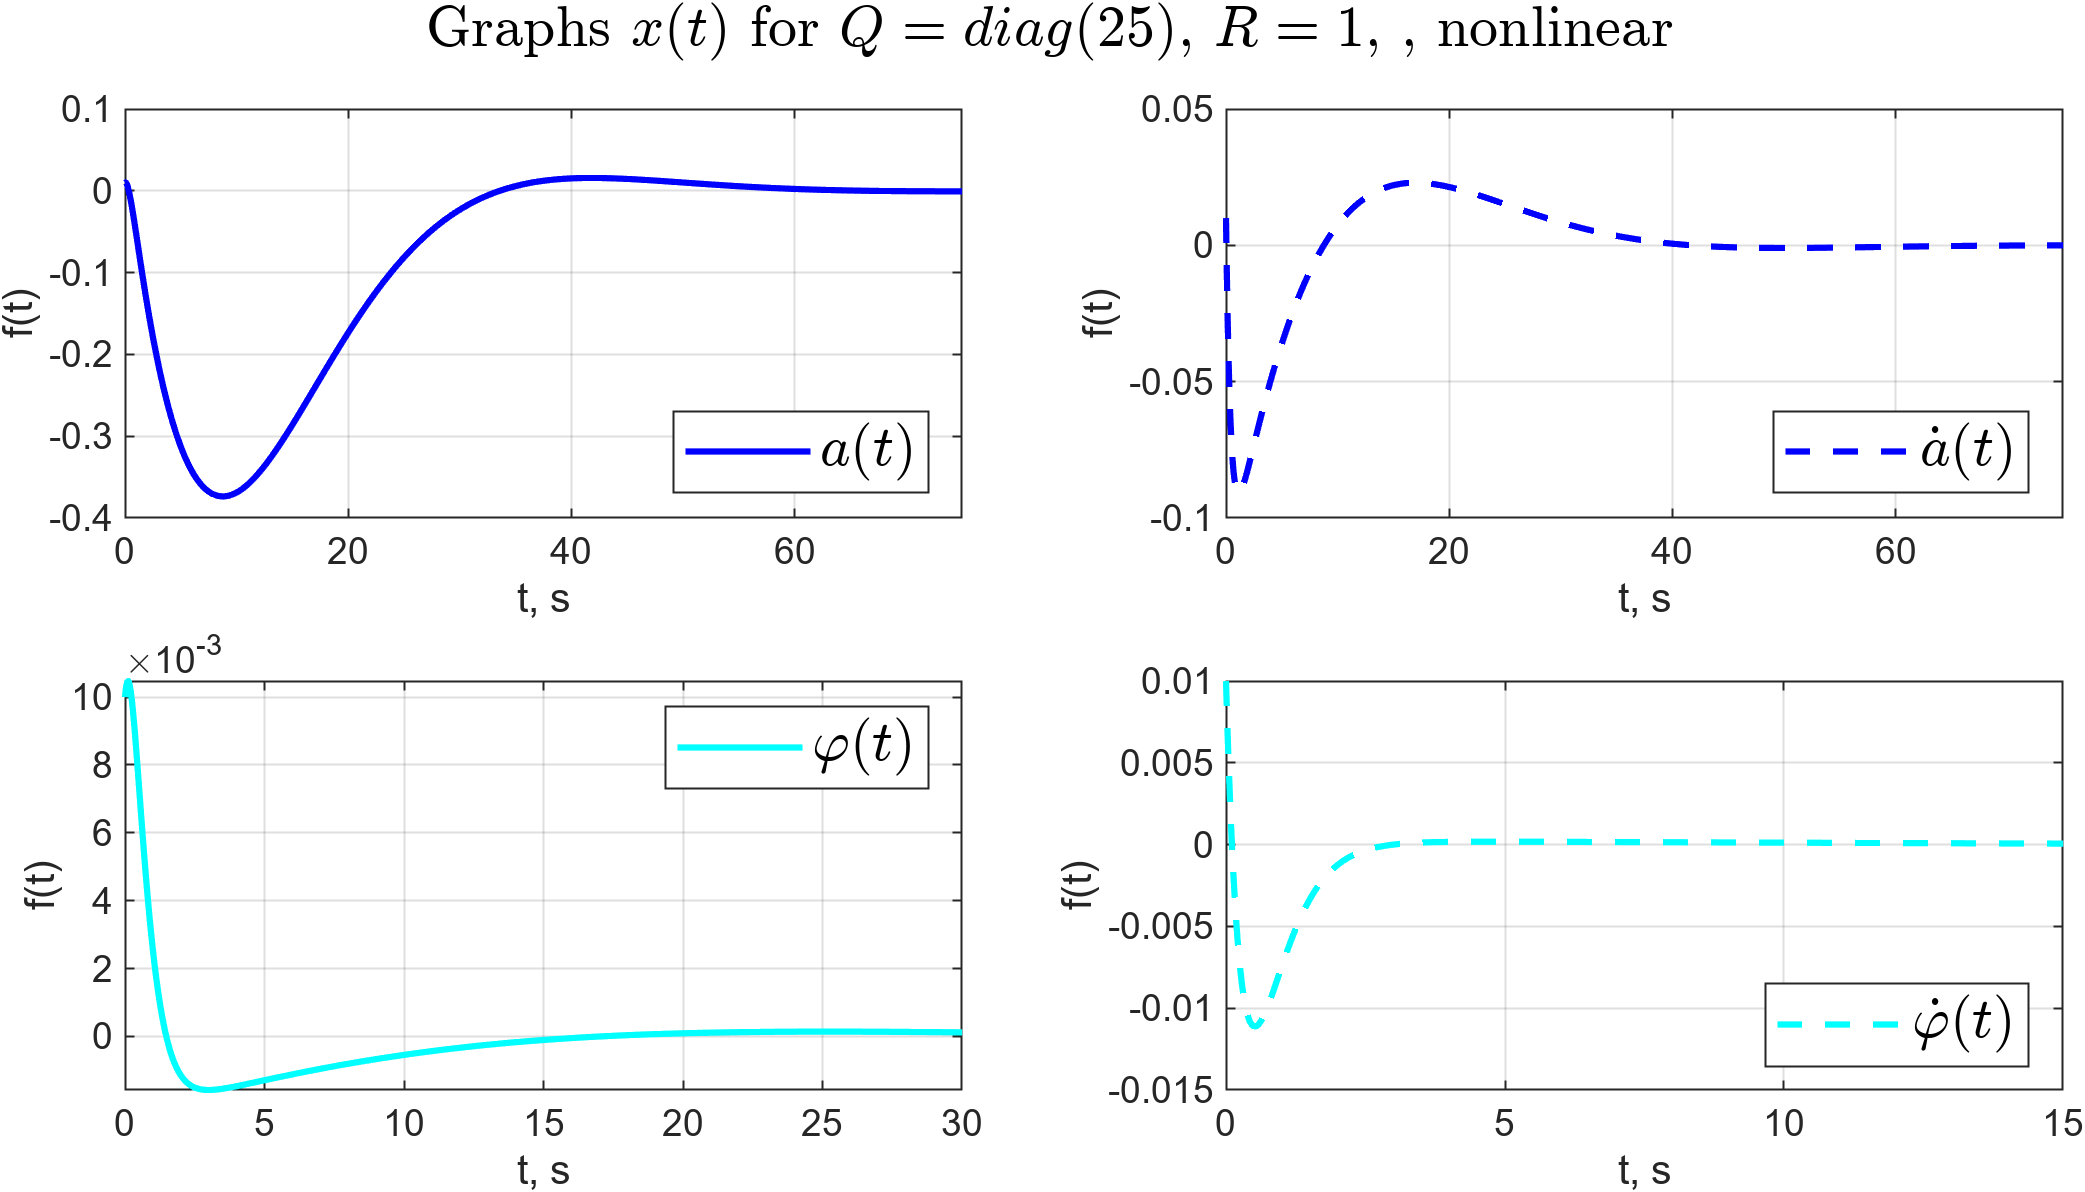
\includegraphics[width=1\linewidth]{pic_fix/6_2_Q_25_R_1_x.png}}
	\caption{Графики компонент вектора состояния системы при $Q=diag(25)$, $R=1$.}
	\label{6_2_Q_25_R_1_x}
\end{figure}

\begin{figure}[!h]
	\center{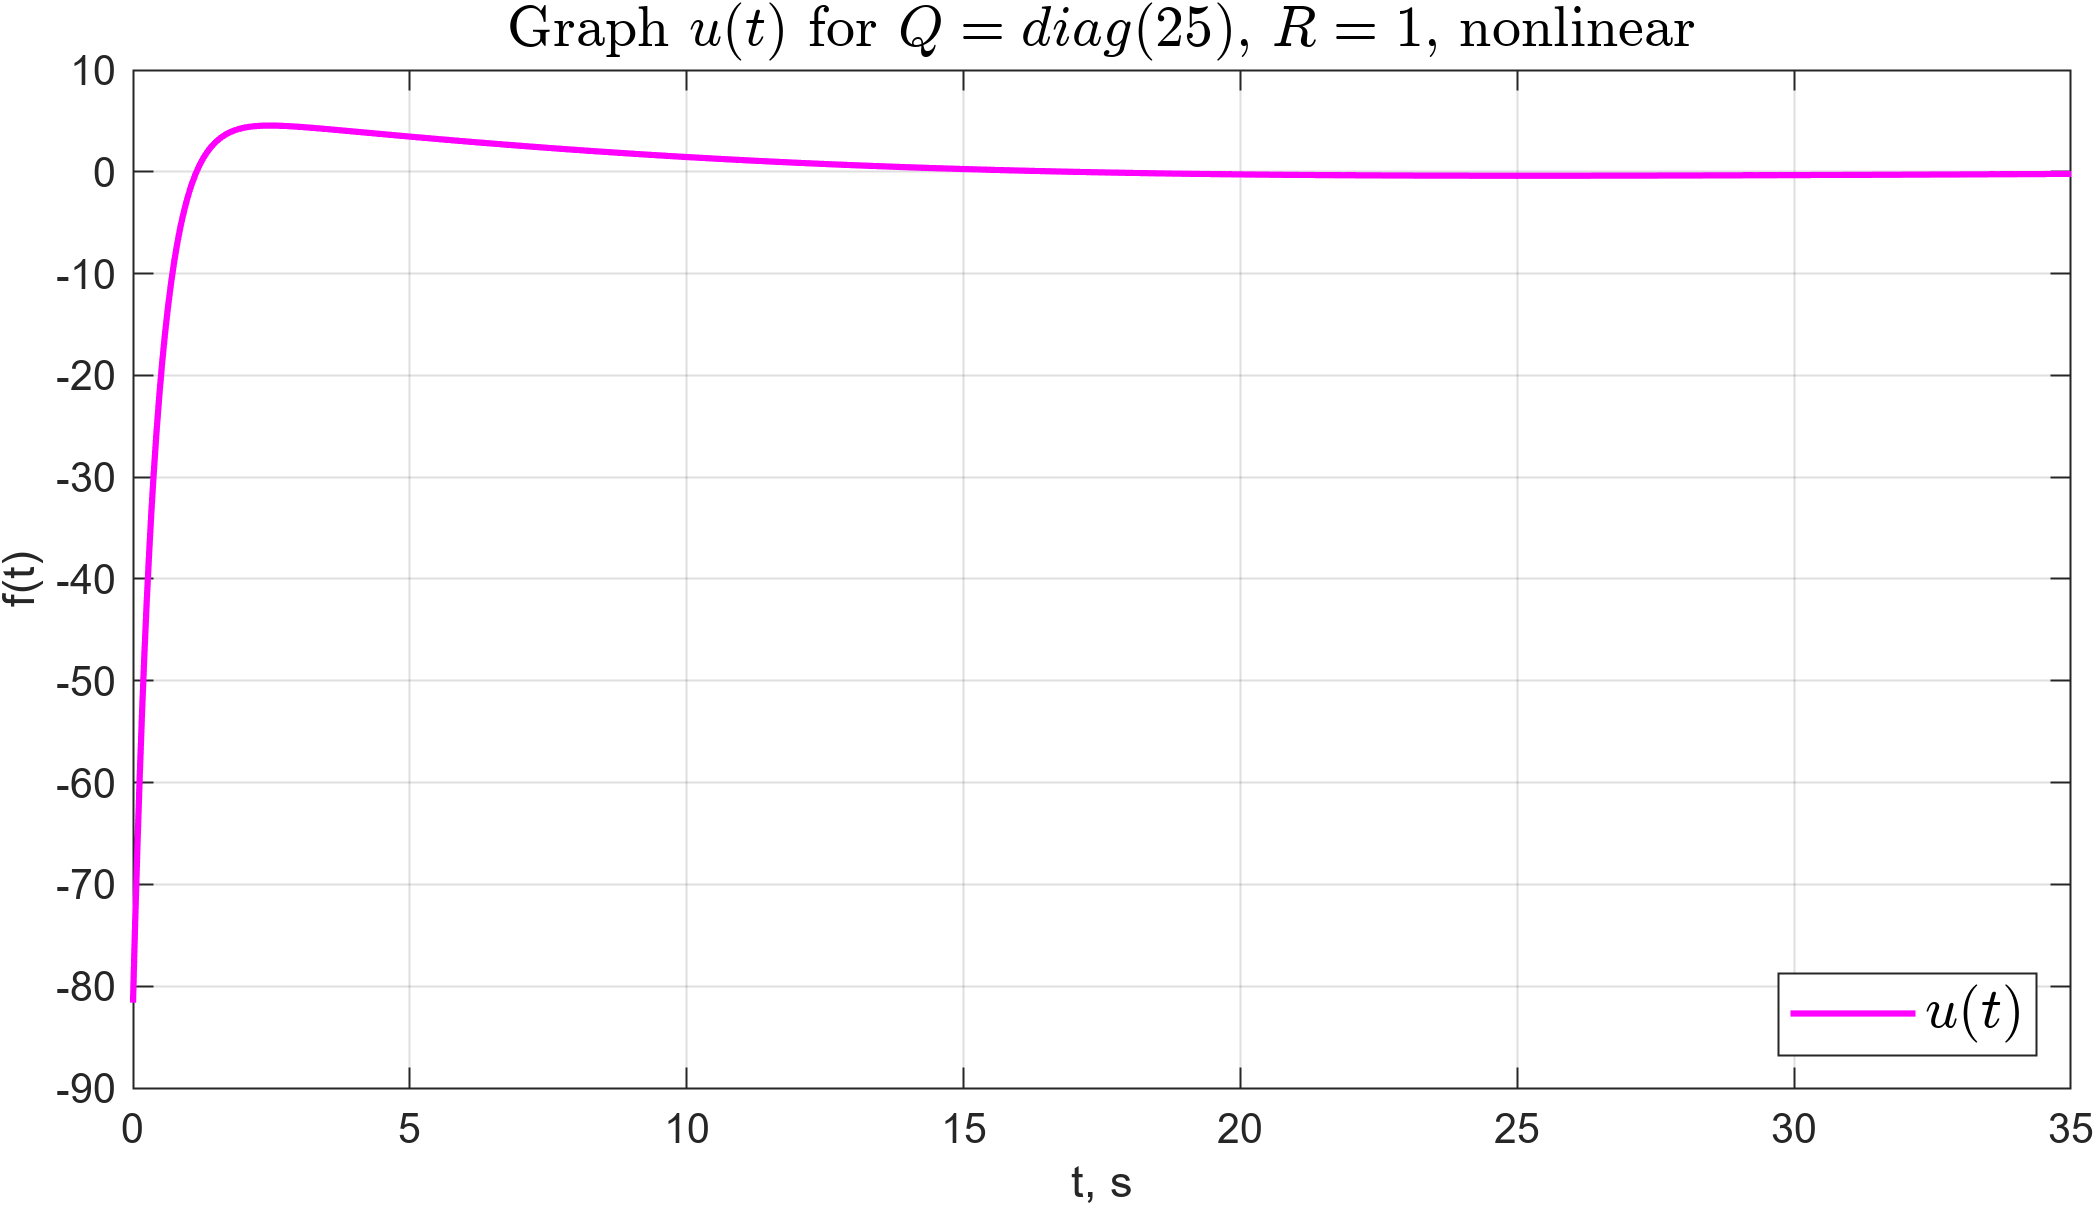
\includegraphics[width=1\linewidth]{pic_fix/6_2_Q_25_R_1_u.png}}
	\caption{График $u(t)$ при $Q=diag(25)$, $R=1$.}
	\label{6_2_Q_25_R_1_u}
\end{figure}


% Q=1 R=1
\begin{figure}[!h]
	\center{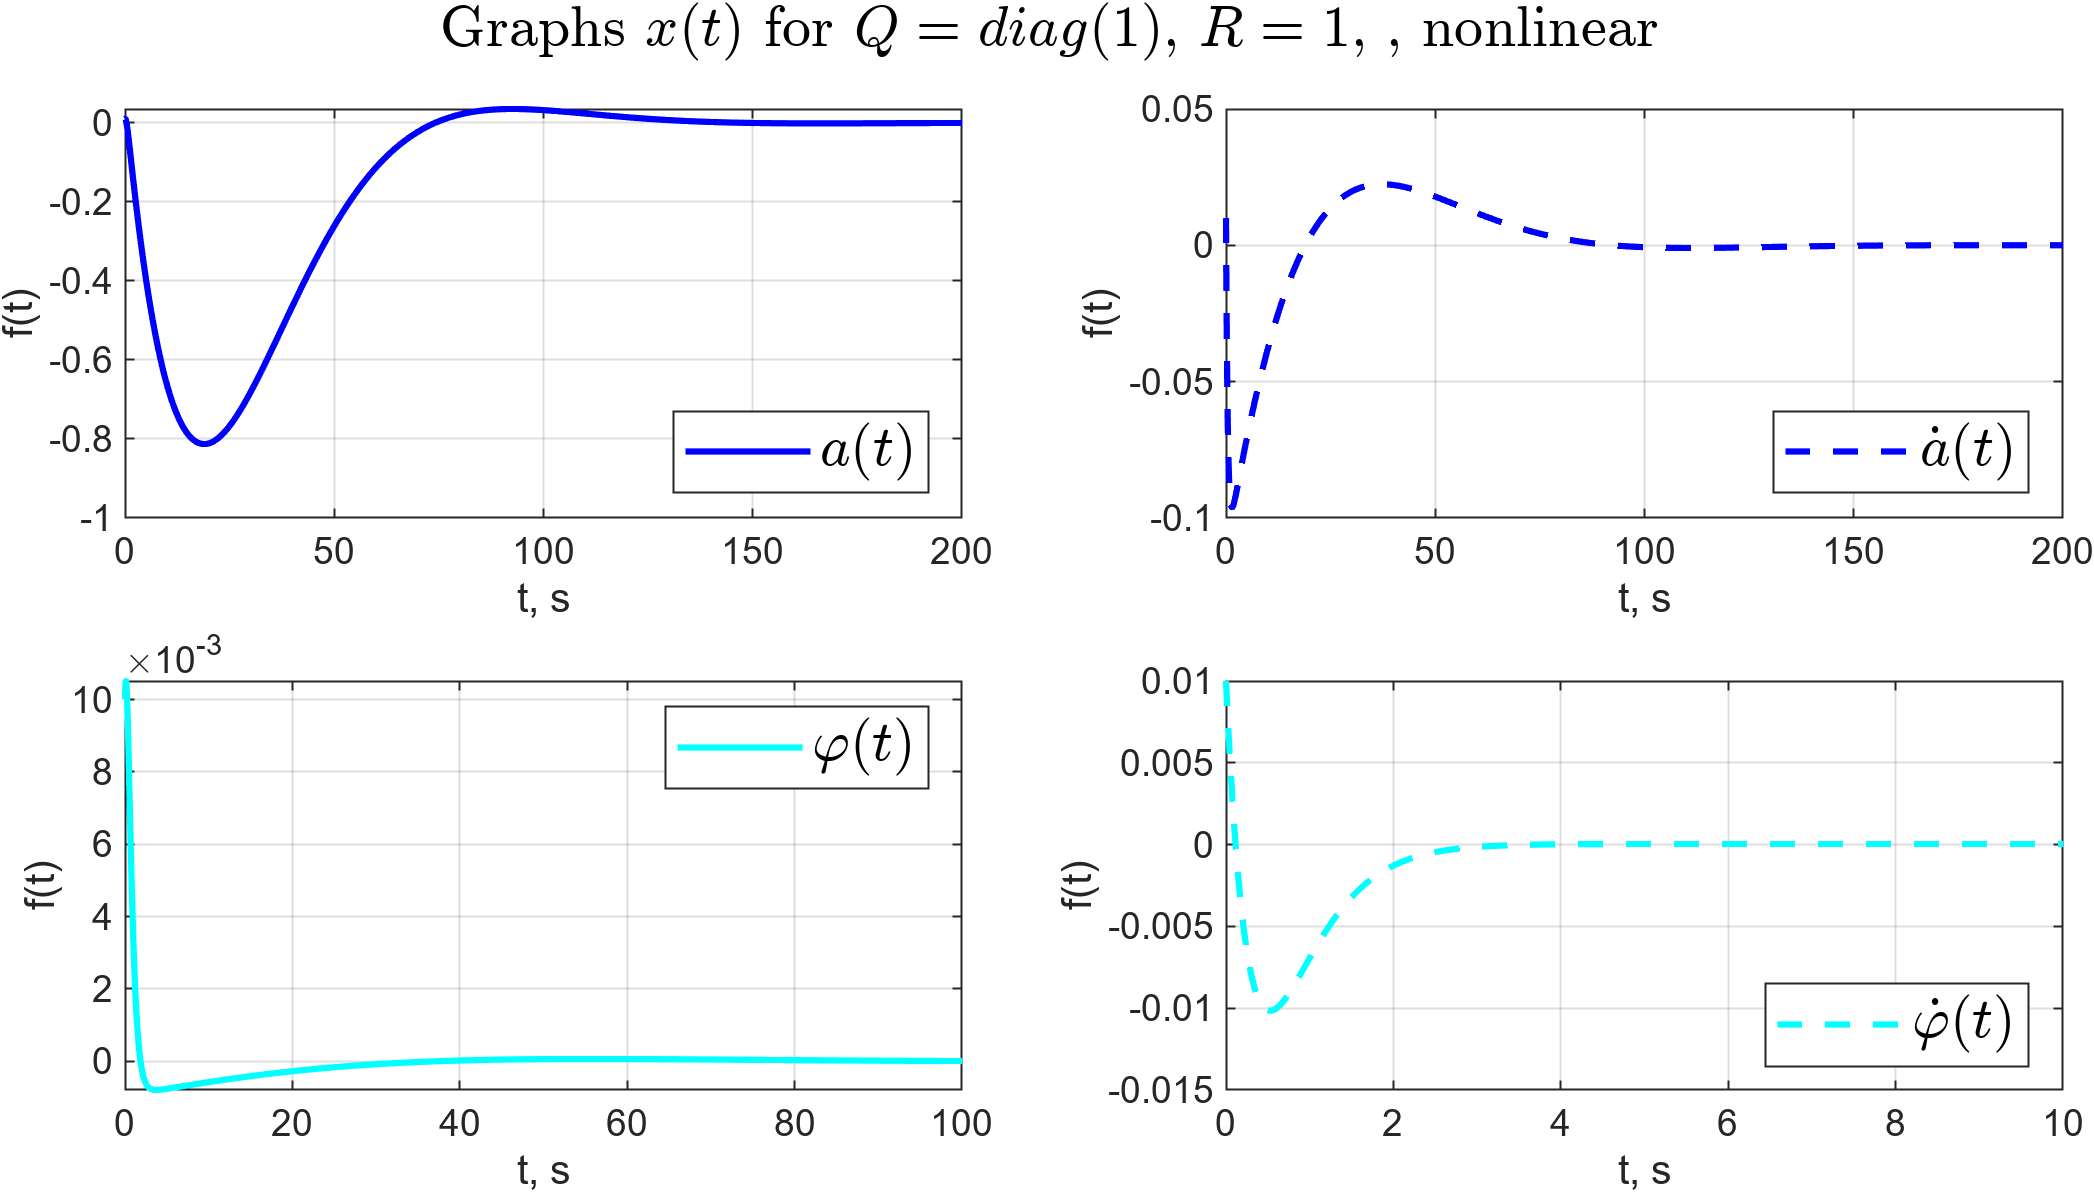
\includegraphics[width=1\linewidth]{pic_fix/6_2_Q_1_R_1_x.png}}
	\caption{Графики компонент вектора состояния системы при $Q=diag(1)$, $R=1$.}
	\label{6_2_Q_1_R_1_x}
\end{figure}

\begin{figure}[!h]
	\center{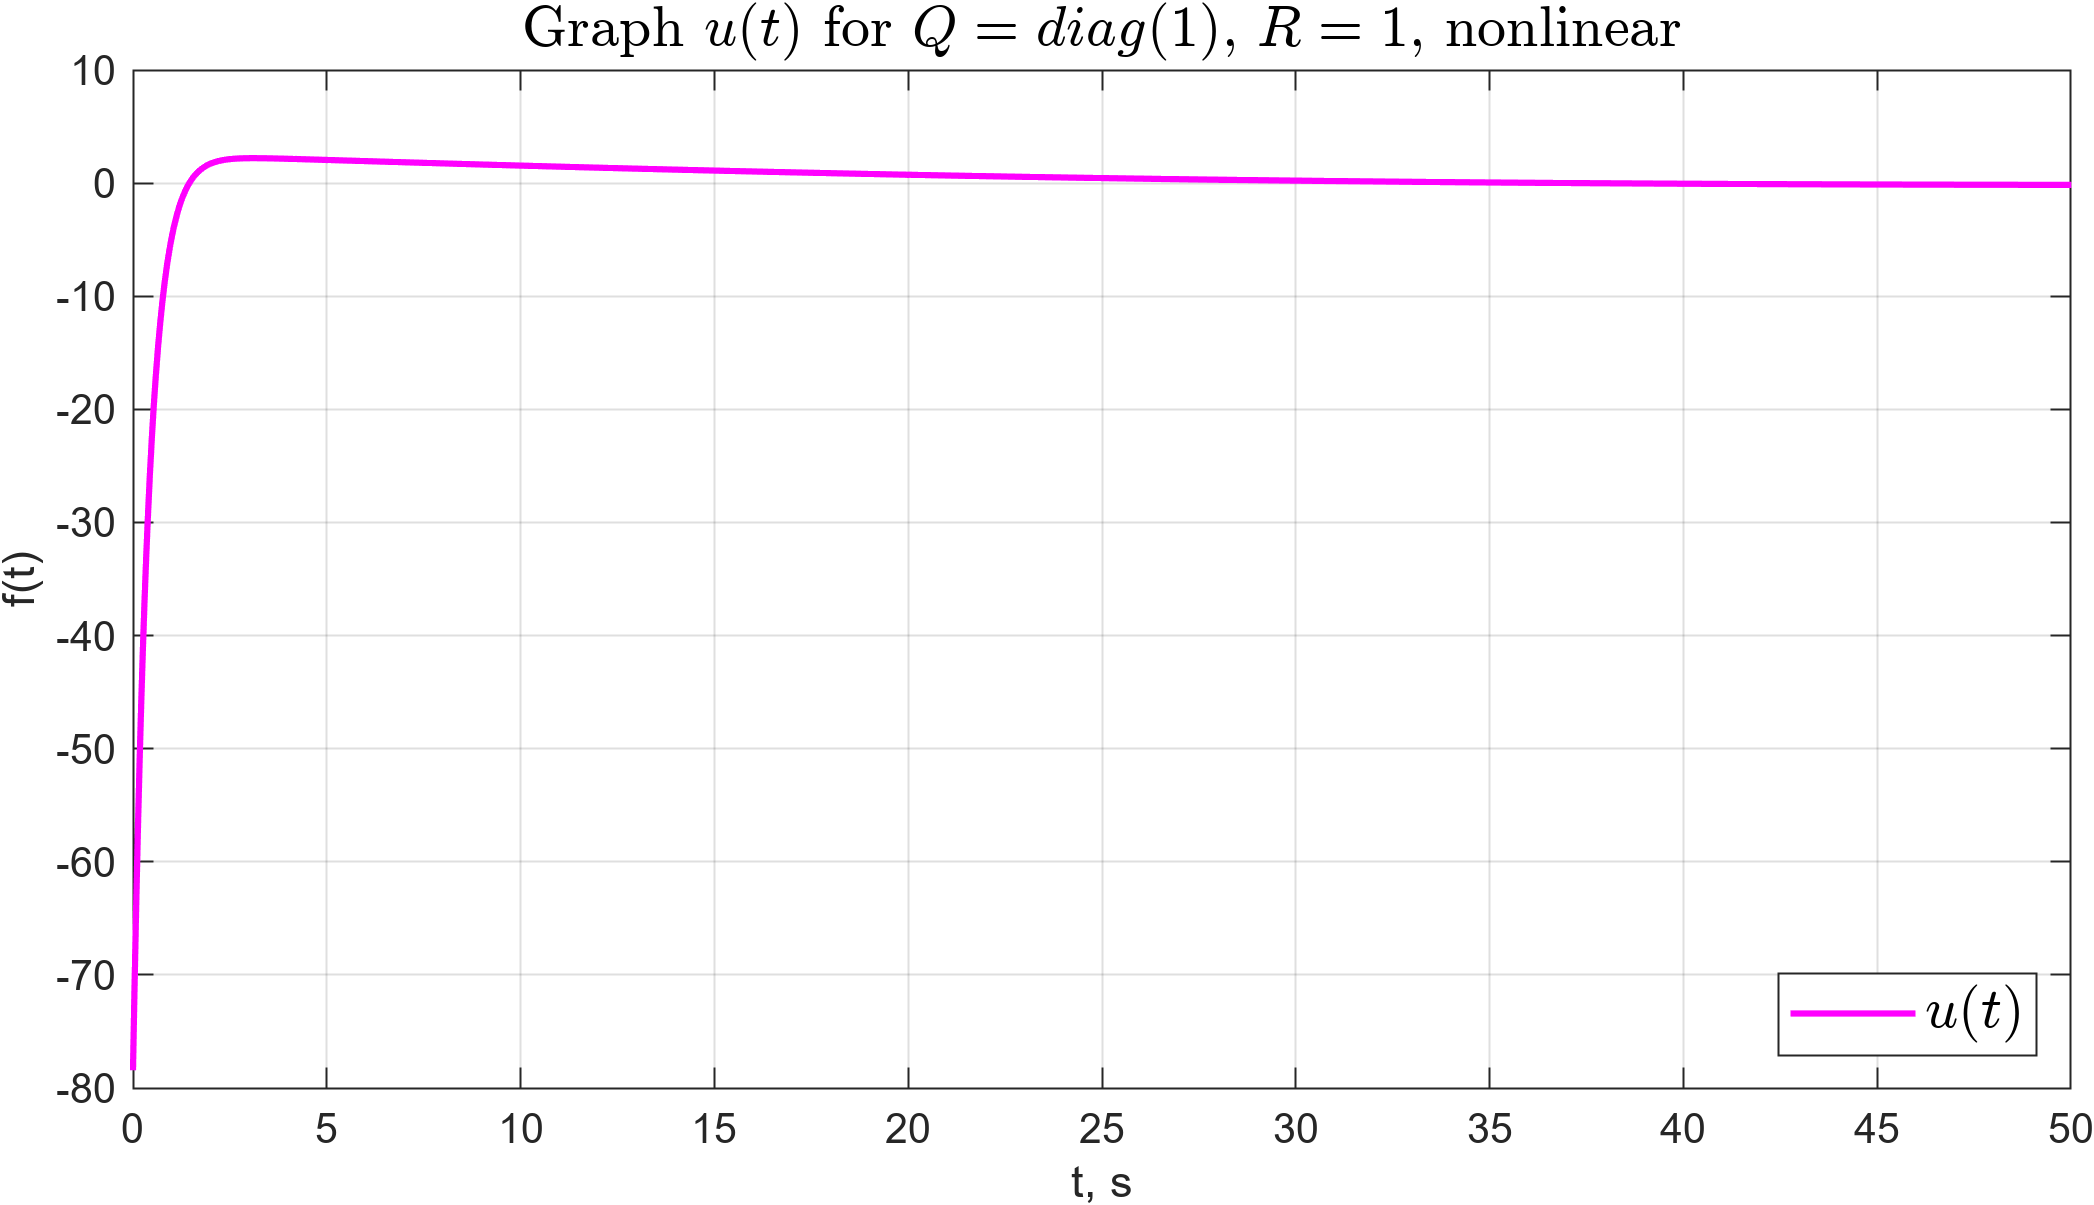
\includegraphics[width=1\linewidth]{pic_fix/6_2_Q_1_R_1_u.png}}
	\caption{График $u(t)$ при $Q=diag(1)$, $R=1$.}
	\label{6_2_Q_1_R_1_u}
\end{figure}


\newpage
\,
\newpage
\,
\newpage
\,
\newpage
\,
\newpage
\,
\newpage

Заметим, что для двух наборов, состоящих из одинаковых $Q$ и $R$, показатели $\max |\varphi|$, $\max |a|$ и $\max |u|$ для одного набора совпадают с соответствующими показателями другого набора. Уменьшение $\max |a|$ происходит одновременно с повышением $\max |u|$.

\section{Синтез фильтра Калмана}
Синтезируем фильтр Калмана в непрерывном времени на основе линейной модели (\ref{1_model_lin}) и применим его для оценки вектора состояния нелинейной системы (\ref{1_model_full}).

Запишем систему с учетом белых шумов $f$ и $\xi$

\begin{equation}
	\begin{cases}
		\dot{x} = Ax + Bu + f,\\
		y = Cx + \xi
	\end{cases}
\end{equation}
Пусть $f(t) \sim \mathcal{N}(0,1)$, $\xi (t) \sim \mathcal{N}(0,0.5)$, тогда выбор матриц $Q$ и $R$ основывается на заданной дисперсии для помех и шумов

\begin{equation}
	\begin{cases}
		E \left( f(t) f^T(t) \right) = \delta (t - \tau)
		\begin{bmatrix}
			\sigma^2_1 & \sigma_{12} & \sigma_{13} & \sigma_{14}\\
			\sigma_{21} & \sigma^2_{2} & \sigma_{23} & \sigma_{24}\\
			\sigma_{31} & \sigma_{32} & \sigma^2_{3} & \sigma_{34}\\
			\sigma_{41} & \sigma_{42} & \sigma_{43} & \sigma^2_{4}
		\end{bmatrix} = \delta(t-\tau) Q_L\\\\
		E \left( \xi(t) \xi^T(t) \right) =
		\delta (t - \tau)
		\begin{bmatrix}
			\sigma^2_1 & \sigma_{12}\\
			\sigma_{21} & \sigma^2_{2} 
		\end{bmatrix} = \delta(t-\tau) R_L
	\end{cases}
\end{equation}
С учетом $ f(t) \sim \mathcal{N}(0,0.1)$ и $ \xi(t)  \sim \mathcal{N}(0,0.01)$ получаем

\begin{equation}
	Q = \begin{bmatrix}
		0.1 & 0 & 0 & 0\\
		0 & 0.1 & 0 & 0\\
		0 & 0 & 0.1 & 0\\
		0 & 0 & 0 & 0.1
	\end{bmatrix}, \, \, \, 
	R=
	\begin{bmatrix}
		0.01 & 0\\
		0 & 0.01
	\end{bmatrix}
\end{equation}




Запишем соответствующее уравнение Риккати

\begin{equation}
	\begin{cases}
		PA^T+AP+Q-\nu PC^TR^{-1}CP=0,\\
		L = -PC^TR^{-1}
	\end{cases}
\end{equation}

Запишем условия существования $P \succ 0$: $Q \succeq 0$, $R \succ 0$, $(C,A)$--обнаруживаема, $(A,Q)$ -- управляема, заметим, что все условия выполнены.

Найдем значение матрицы $L$

\begin{equation}
	L = \begin{bmatrix}
		    -4.0417 &  -0.0563\\
		 -3.1691 &  -0.3975\\
		 -0.0563 &  -5.9121\\
		 -0.1632 & -12.4782
	\end{bmatrix}
\end{equation}

Выберем из предыдущего пункта регулятор с матрицей $K$, соответствующей $Q_K=diag(10)$, $R_K=1$

 \begin{equation}
	K = \begin{bmatrix}
		3.2 &   44.3 &  -5720.8   &-2369.3
	\end{bmatrix}
\end{equation}

и выполним моделирование

\begin{figure}[!h]
	\center{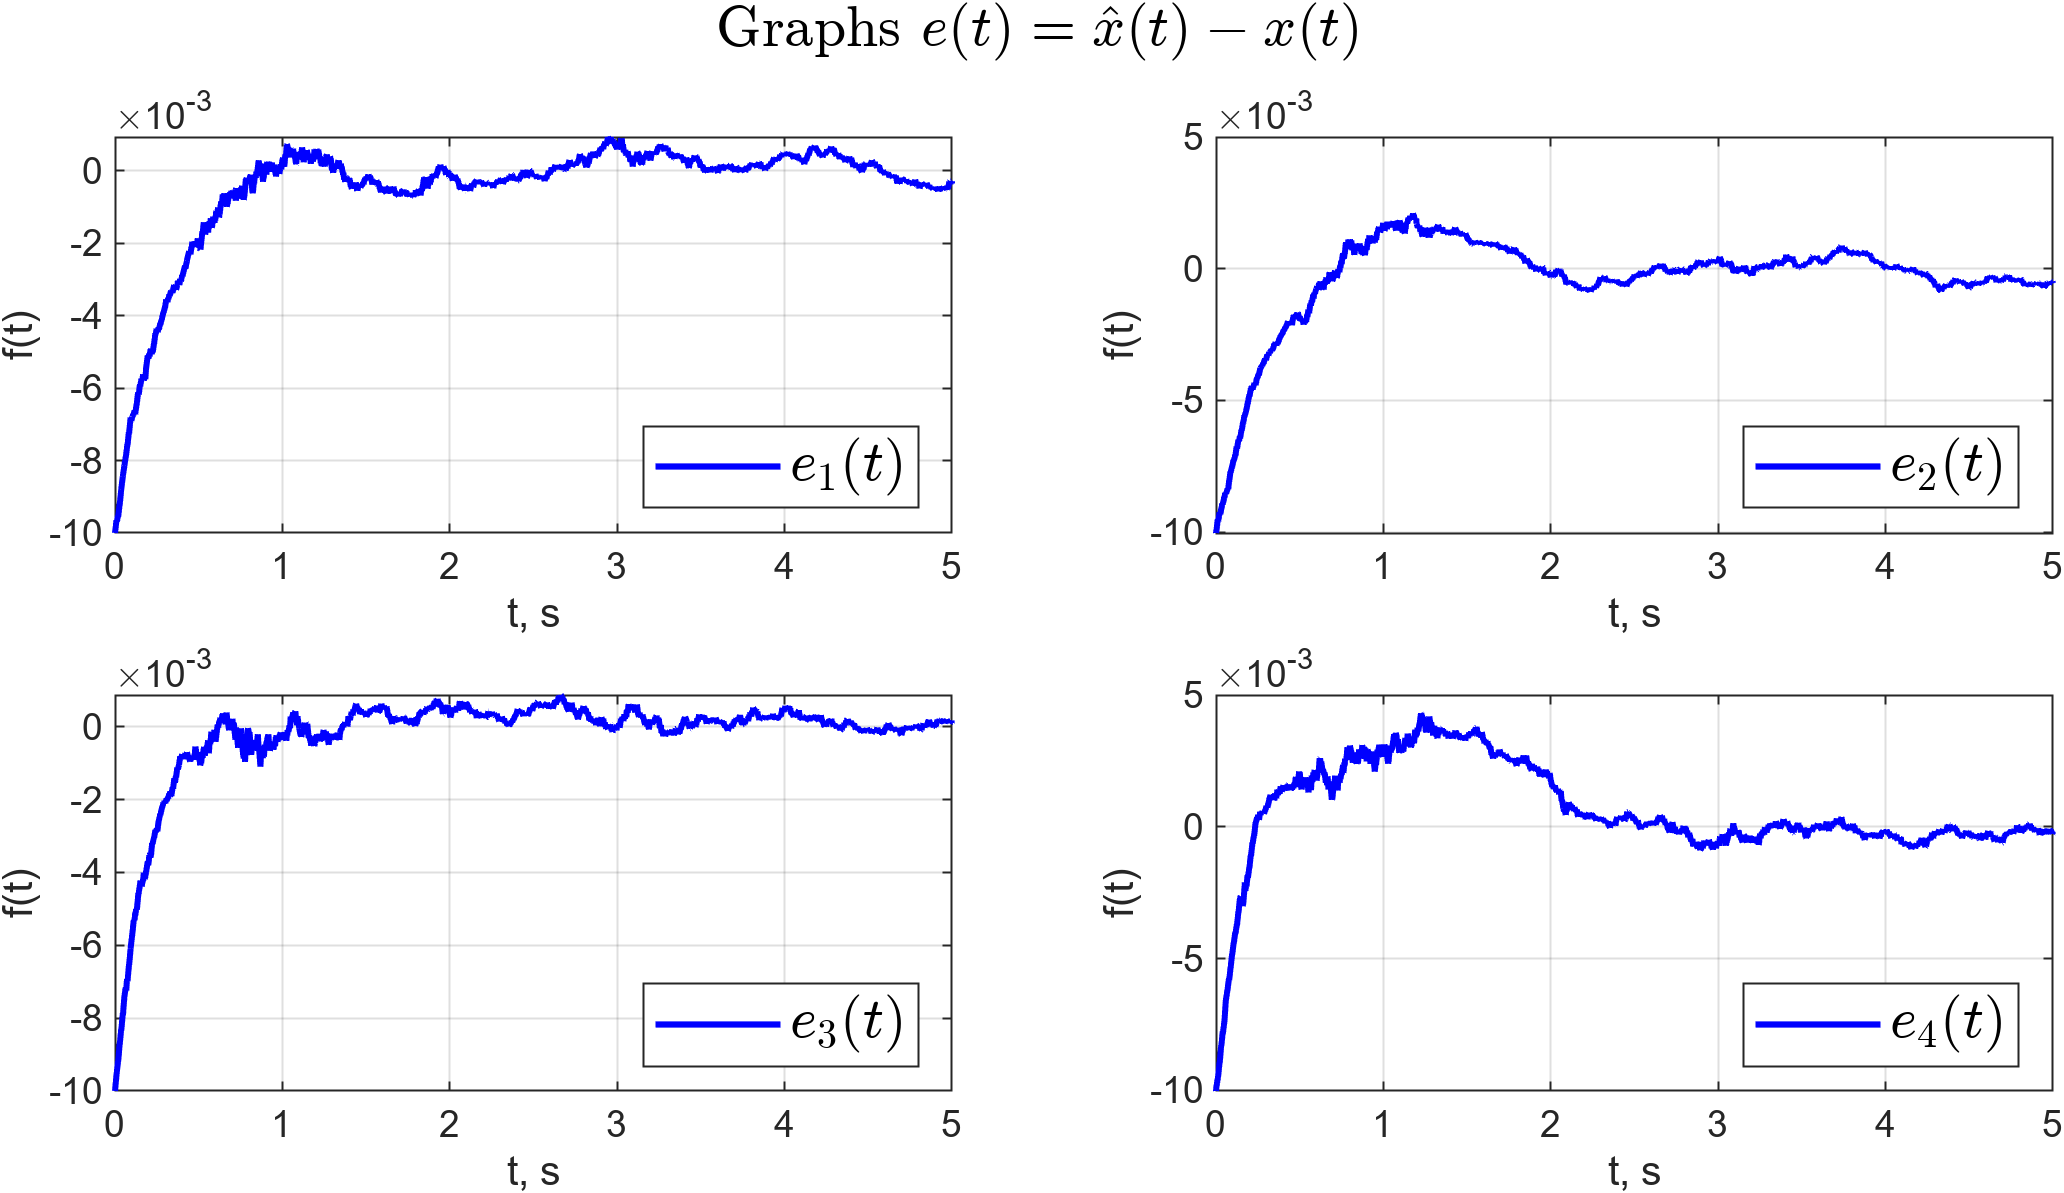
\includegraphics[width=1\linewidth]{pic2/6_kalm_e_1.png}}
	\caption{Графики $e(t) = \hat{x}-x(t)$ для нелинейной системы.}
	\label{6_kalm_e_1}
\end{figure}

\begin{figure}[!h]
	\center{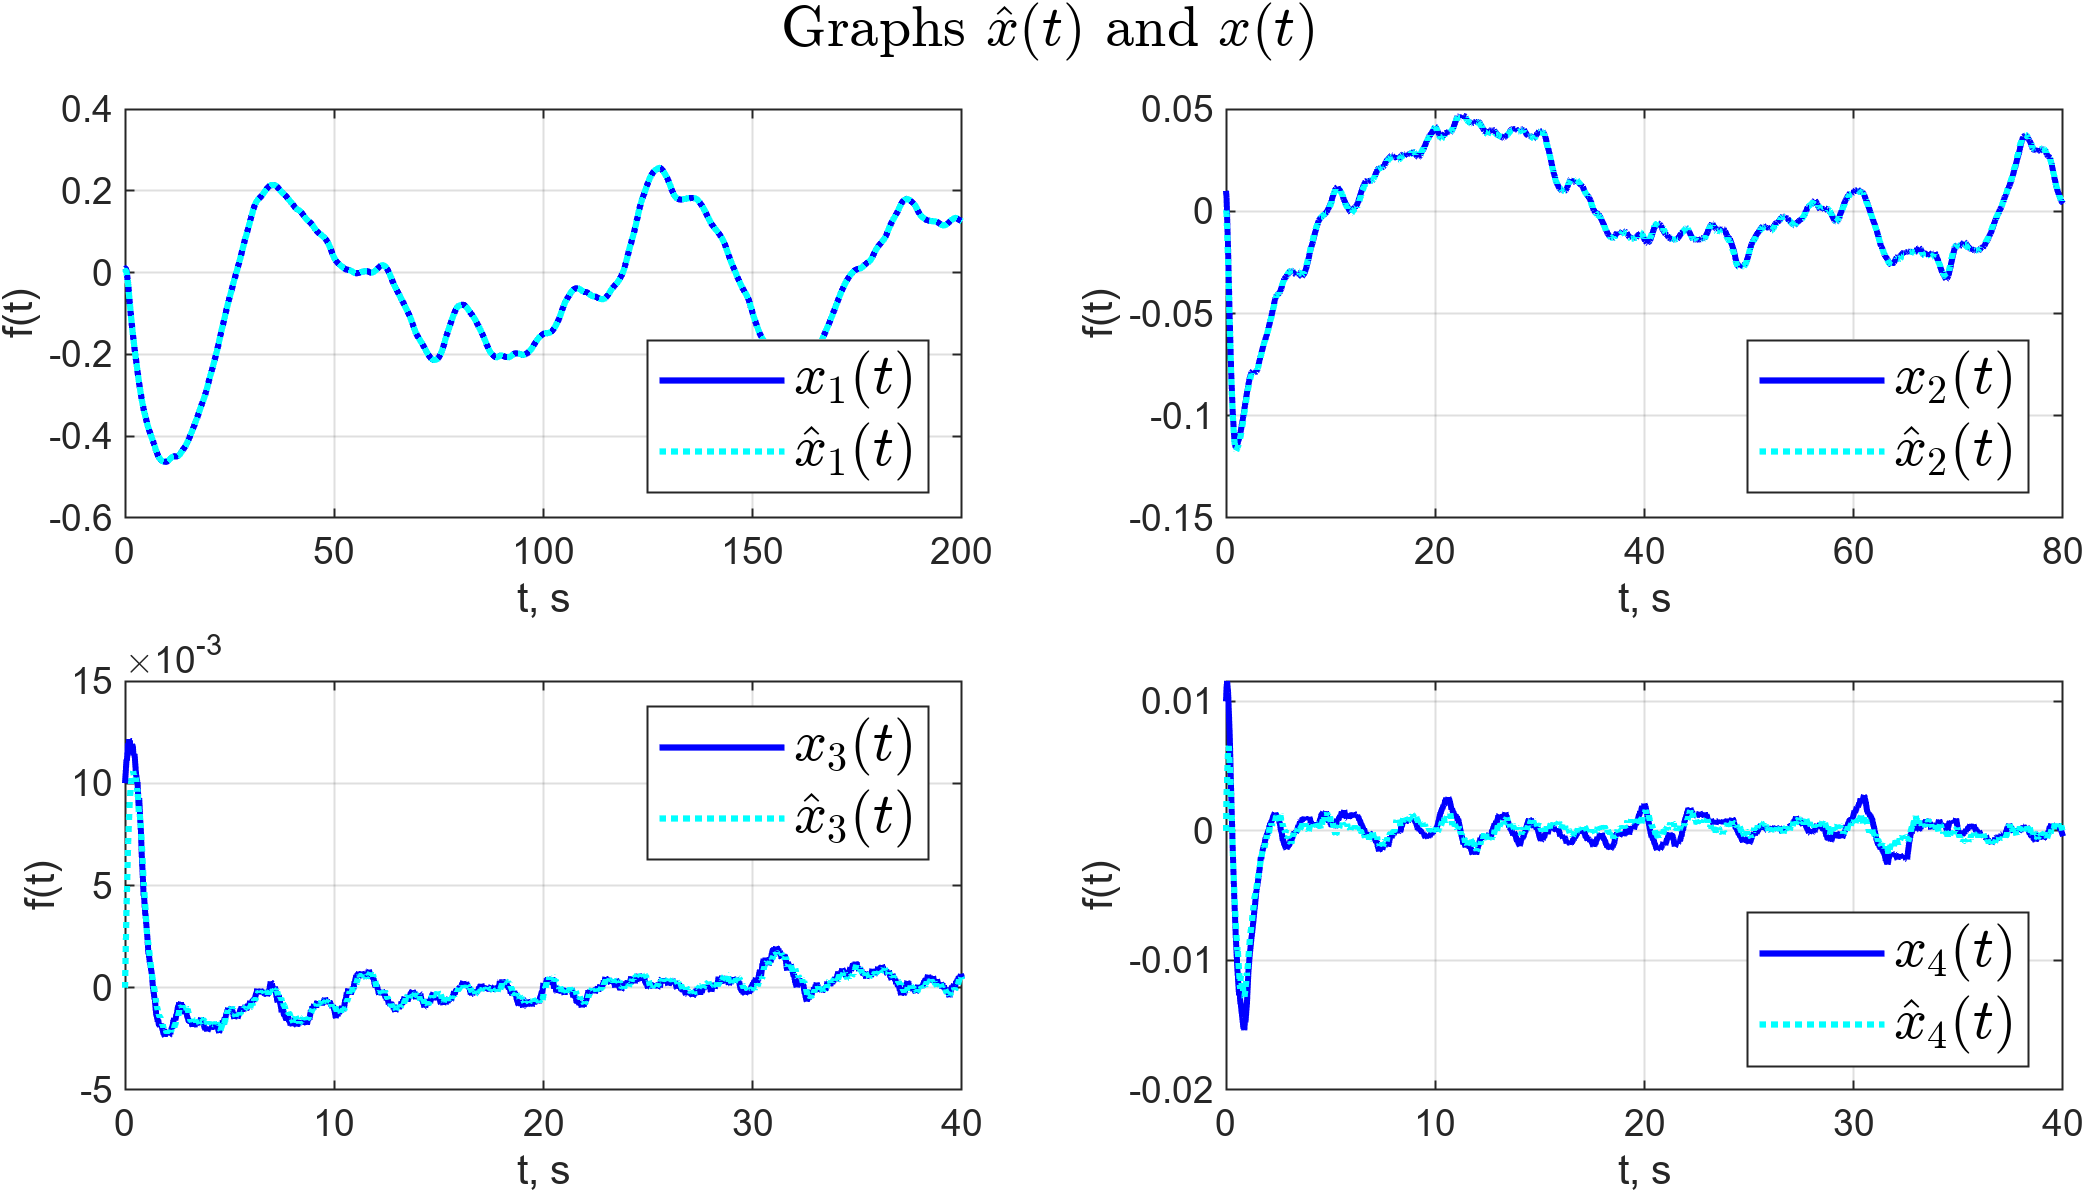
\includegraphics[width=1\linewidth]{pic2/6_kalm_x_1.png}}
	\caption{Графики $\hat{x}$ и $x(t)$ для нелинейной системы.}
	\label{6_kalm_x_1}
\end{figure}

Как видим, фильтр работает для нелинейной системы (рисунки \ref{6_kalm_e_} и \ref{6_kalm_x_}).

\section{LQG для линейной модели}
Применим LQR-регулятор совместно с фильтром Калмана для управления линейной моделью

\begin{equation}
	\begin{cases}
\dot{x} = Ax + Bu + Df,\\
y = Cx + \xi,
	\end{cases}
\end{equation}
в которой зададим сигналы $f \sim \mathcal{N} (0, 0.1)$ и $\xi\sim \mathcal{N} (0, 0.01)$ как белый шум соответствующей интенсивности, то есть наблюдатель будет взят из предыдущего пункта. 

Регулятор найдем, задавшись следующими матрицами

\begin{equation}
	Q = \begin{bmatrix}
		10^5 & 0 & 0 & 0\\
		0 & 10 & 0 & 0\\
		0 & 0 & 10 & 0\\
		0 & 0 & 0 & 10
	\end{bmatrix}, \, \, R=1
\end{equation}

\begin{equation}
K= \begin{bmatrix}
	100&371&-7612.8&-3162.3
\end{bmatrix}
\end{equation}

\begin{figure}[!h]
	\center{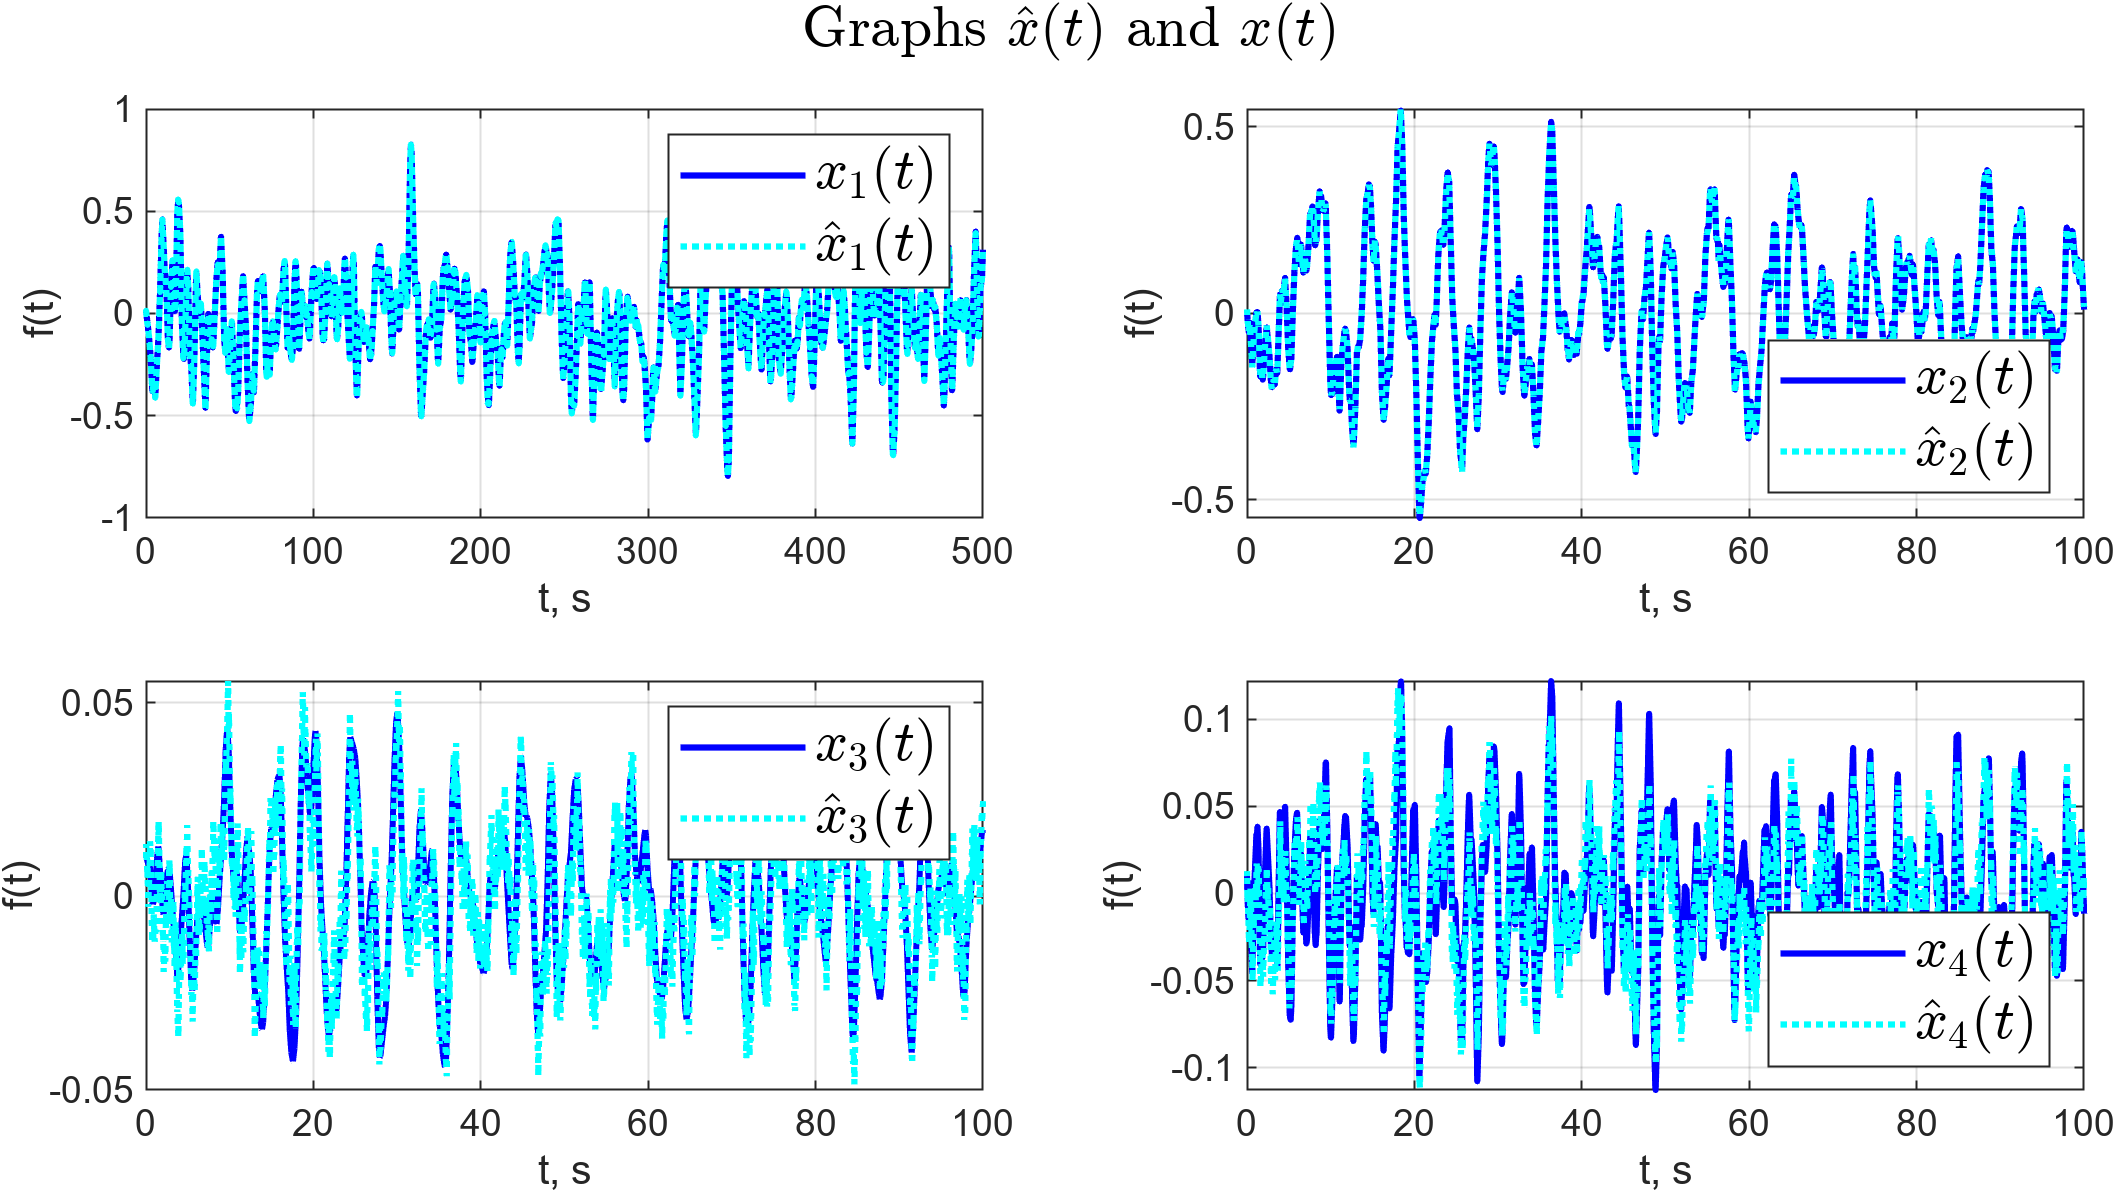
\includegraphics[width=1\linewidth]{pic2/6_lqg_lin2.png}}
	\caption{Графики $\hat{x}$ и $x(t)$ для линейной системы.}
	\label{6_lqg_lin2}
\end{figure}

\begin{figure}[!h]
	\center{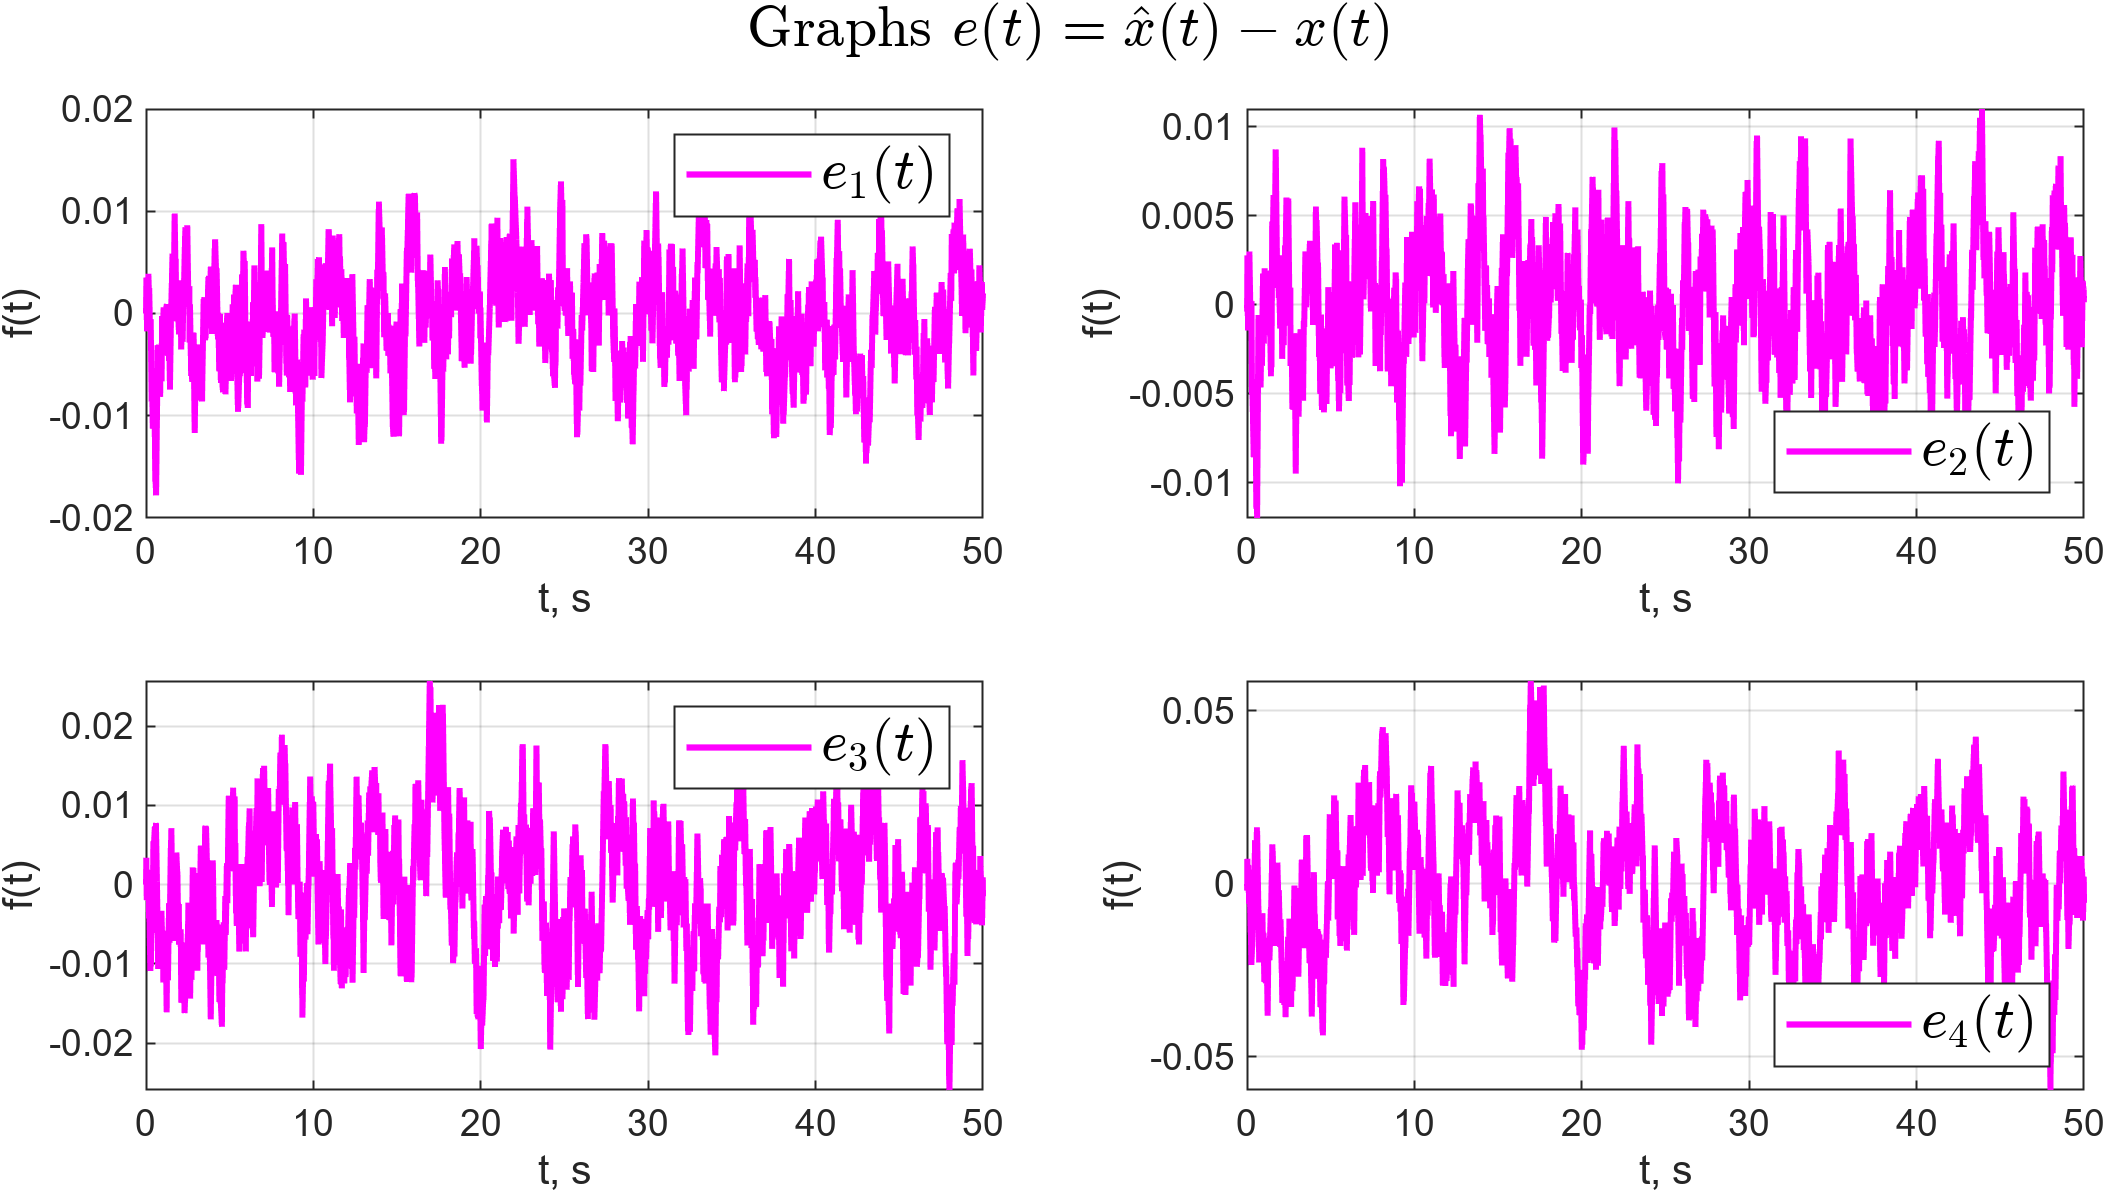
\includegraphics[width=1\linewidth]{pic2/6_lqg_lin2_e.png}}
	\caption{Графики $e(t) =\hat{x}- x(t)$ для линейной системы.}
	\label{6_lqg_lin2_e}
\end{figure}

Можно заметить, что компоненты вектора-состояния линейной системы колеблются около точки равновесия системы (рисунок \ref{6_lqg_lin2}). Отклонения от нуля в данном случае можно объеснить воздействием белого шума.


\section{LQG для нелинейной модели}

Применим LQR-регулятор и фильтр Калмана, синтезированные в прошлом пункте для управления нелинейной моделью.

\begin{figure}[!h]
	\center{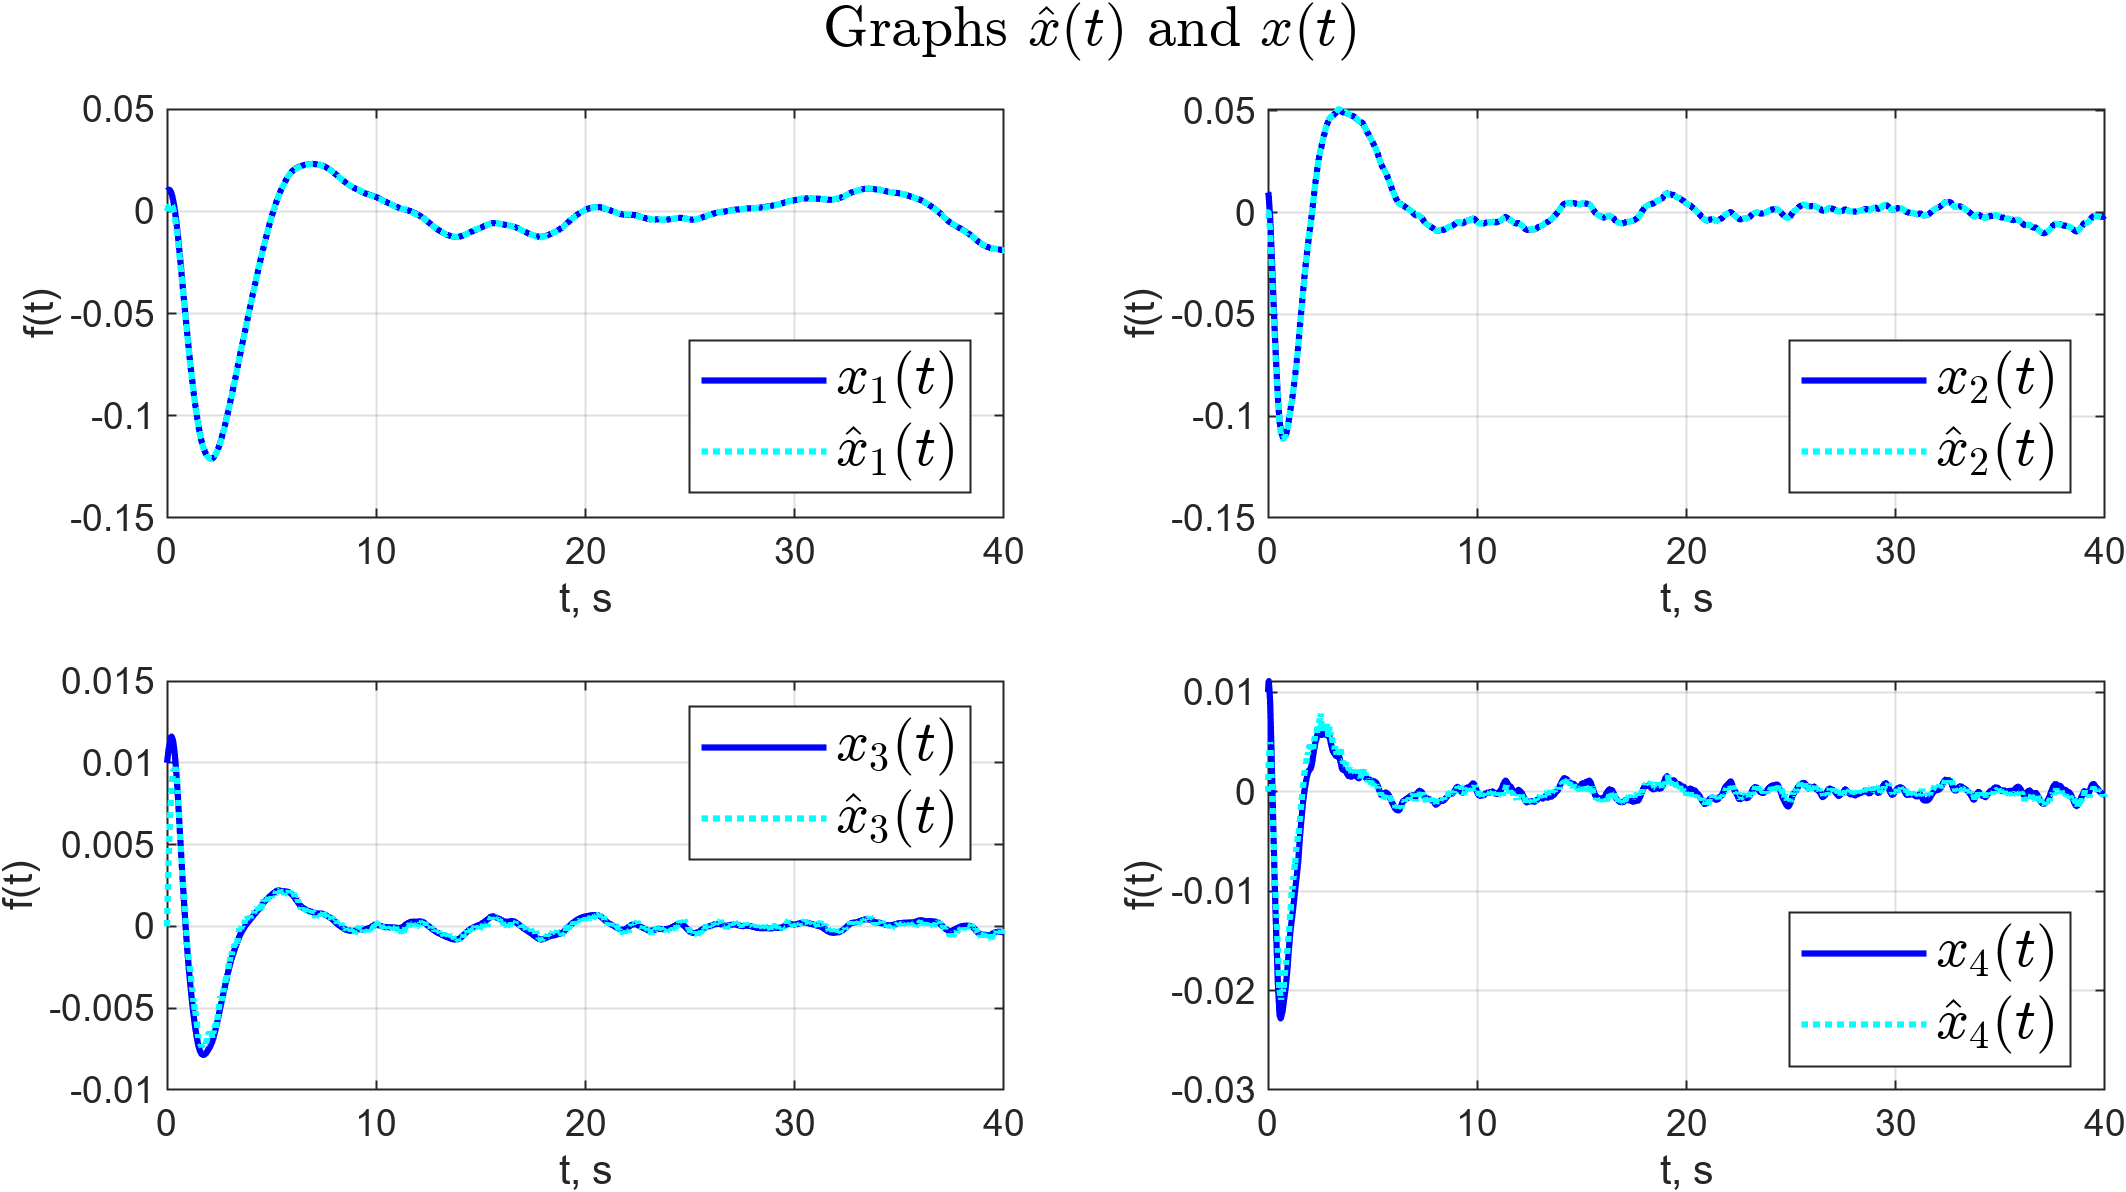
\includegraphics[width=1\linewidth]{pic2/6_lqg_nonlin2_x.png}}
	\caption{Графики $\hat{x}$ и $x(t)$ для нелинейной системы.}
	\label{6_lqg_nonlin2_x}
\end{figure}

\begin{figure}[!h]
	\center{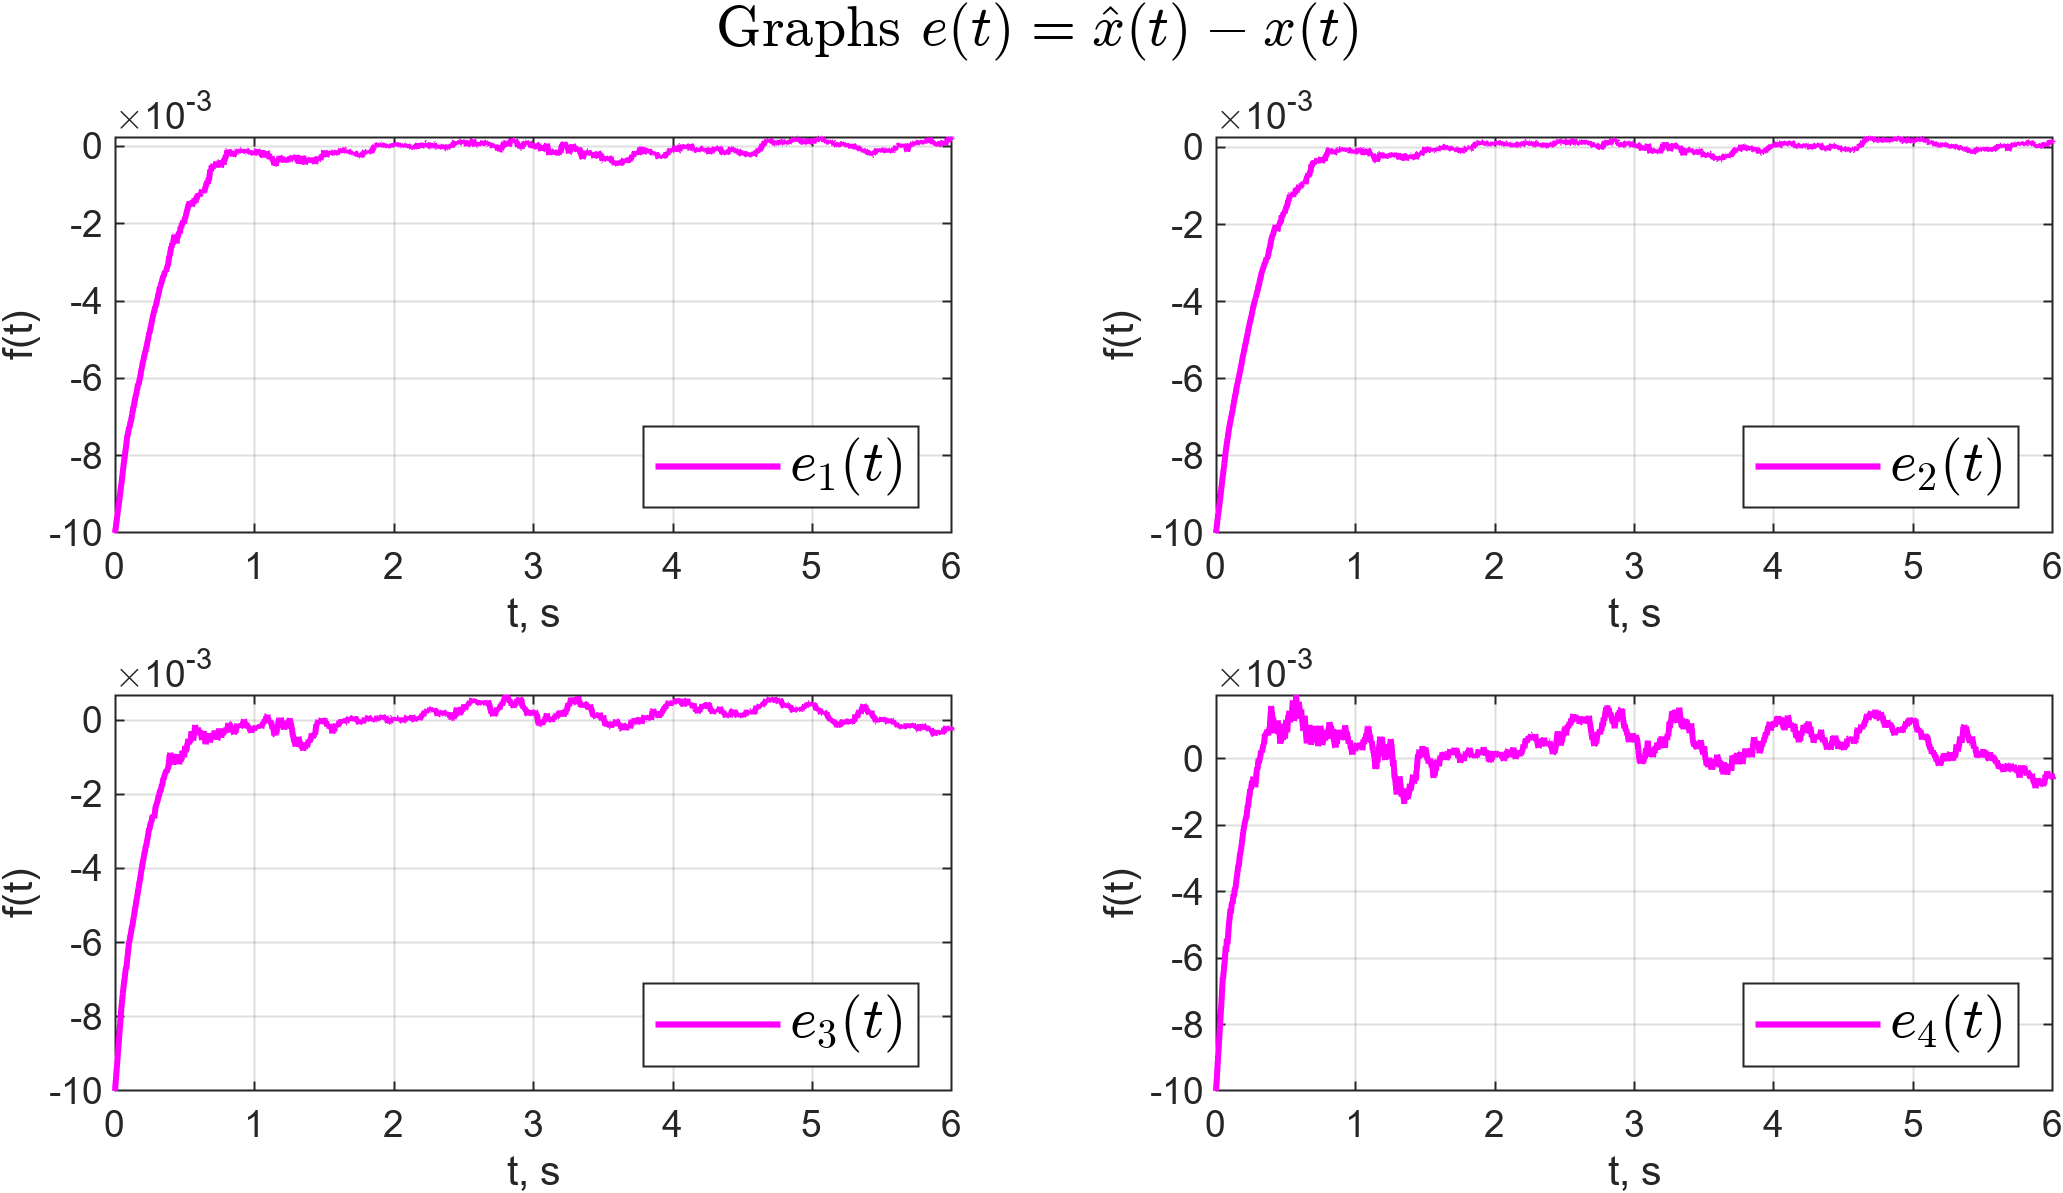
\includegraphics[width=1\linewidth]{pic2/6_lqg_nonlin2_e.png}}
	\caption{Графики $x(t) = \hat{x}-x(t)$ для нелинейной системы.}
	\label{6_lqg_nonlin2_e}
\end{figure}

\endinput